%%%%%%%% ICML 2026 EXAMPLE LATEX SUBMISSION FILE %%%%%%%%%%%%%%%%%

\documentclass{article}

% Recommended, but optional, packages for figures and better typesetting:
\usepackage{microtype}
\usepackage{graphicx}
\usepackage{subcaption}
\usepackage{booktabs} % for professional tables
\usepackage{makecell} % for multi-line table headers
\usepackage{multirow} % for multi-row table cells
\usepackage{longtable} % for tables that span multiple pages
\usepackage{enumitem} % for compact lists
\usepackage{minted} % for code/prompt blocks with syntax highlighting

% Shortcuts for benchmark names
\newcommand{\tauvoice}{$\tau$-Voice}
\newcommand{\taubench}{$\tau$-bench}
\newcommand{\tautwobench}{$\tau^2$-bench}

% Author comments: usage \authornote{Name}{Comment text}
% Set to false to hide all author notes (for final submission)
\newif\ifshownotes
% \shownotestrue  % Change to \shownotesfalse to hide all notes
\shownotesfalse
\newcommand{\authornote}[2]{\ifshownotes\todo[color=orange!40,inline]{\textbf{#1:} #2}\fi}

% hyperref makes hyperlinks in the resulting PDF.
% If your build breaks (sometimes temporarily if a hyperlink spans a page)
% please comment out the following usepackage line and replace
% \usepackage{icml2026} with \usepackage[nohyperref]{icml2026} above.
\usepackage{hyperref}
\usepackage{xurl}  % Allow URLs to break at any character

% Attempt to make hyperref and algorithmic work together better:
\newcommand{\theHalgorithm}{\arabic{algorithm}}

% Use the following line for the initial blind version submitted for review:
\usepackage{icml2026}

% For preprint, use
% \usepackage[preprint]{icml2026}

% If accepted, instead use the following line for the camera-ready submission:
% \usepackage[accepted]{icml2026}

\usepackage{amsmath}
\usepackage{amssymb}
\usepackage{mathtools}
\usepackage{amsthm}


% if you use cleveref..
\usepackage[capitalize,noabbrev]{cleveref}

%%%%%%%%%%%%%%%%%%%%%%%%%%%%%%%%
% THEOREMS
%%%%%%%%%%%%%%%%%%%%%%%%%%%%%%%%
\theoremstyle{plain}
\newtheorem{theorem}{Theorem}[section]
\newtheorem{proposition}[theorem]{Proposition}
\newtheorem{lemma}[theorem]{Lemma}
\newtheorem{corollary}[theorem]{Corollary}
\theoremstyle{definition}
\newtheorem{definition}[theorem]{Definition}
\newtheorem{assumption}[theorem]{Assumption}
\theoremstyle{remark}
\newtheorem{remark}[theorem]{Remark}

% Todonotes is useful during development; simply uncomment the next line
%    and comment out the line below the next line to turn off comments
%\usepackage[disable,textsize=tiny]{todonotes}
\usepackage[textsize=tiny]{todonotes}

% The \icmltitle you define below is probably too long as a header.
% Therefore, a short form for the running title is supplied here:
\icmltitlerunning{$\tau$-Voice}

\begin{document}

\twocolumn[
  \icmltitle{$\tau$-Voice: Benchmarking Full-Duplex Voice Agents on Real-World Domains}

  % It is OKAY to include author information, even for blind submissions: the
  % style file will automatically remove it for you unless you've provided
  % the [accepted] option to the icml2026 package.

  % List of affiliations: The first argument should be a (short) identifier you
  % will use later to specify author affiliations Academic affiliations
  % should list Department, University, City, Region, Country Industry
  % affiliations should list Company, City, Region, Country

  % You can specify symbols, otherwise they are numbered in order. Ideally, you
  % should not use this facility. Affiliations will be numbered in order of
  % appearance and this is the preferred way.
  \icmlsetsymbol{equal}{*}

  \begin{icmlauthorlist}
    \icmlauthor{Soham Ray}{equal,sierra}
    \icmlauthor{Keshav Dhandhania}{equal,sierra}
    \icmlauthor{Victor Barres}{equal,sierra}
    \icmlauthor{Karthik Narasimhan}{princeton}
  \end{icmlauthorlist}

  \icmlaffiliation{sierra}{Sierra.ai, San Francisco, USA}
  \icmlaffiliation{princeton}{Princeton Language and Intelligence, Princeton University}

  \icmlcorrespondingauthor{Victor Barres}{victor@sierra.ai}

  % You may provide any keywords that you find helpful for describing your
  % paper; these are used to populate the "keywords" metadata in the PDF but
  % will not be shown in the document
  \icmlkeywords{Machine Learning, ICML}

  \vskip 0.3in
]

% this must go after the closing bracket ] following \twocolumn[ ...

% This command actually creates the footnote in the first column listing the
% affiliations and the copyright notice. The command takes one argument, which
% is text to display at the start of the footnote. The \icmlEqualContribution
% command is standard text for equal contribution. Remove it (just {}) if you
% do not need this facility.

% Use ONE of the following lines. DO NOT remove the command.
% If you have no special notice, KEEP empty braces:
% \printAffiliationsAndNotice{}  % no special notice (required even if empty)
% Or, if applicable, use the standard equal contribution text:
\printAffiliationsAndNotice{\icmlEqualContribution}

%%%%%%%%%%%%%%%%%%%%%%%%%%%%%%%%%%%%%%%%%%%%%%%%%%%%%%%%%%%%%%%%%%%%%%%%%%%%%%%
% ABSTRACT
%%%%%%%%%%%%%%%%%%%%%%%%%%%%%%%%%%%%%%%%%%%%%%%%%%%%%%%%%%%%%%%%%%%%%%%%%%%%%%%
\begin{abstract}
% Abstract: Keep brief and self-contained, one paragraph, 4-6 sentences.
% Should state: (1) problem/motivation, (2) approach, (3) key results, (4) significance.

Full-duplex voice agents—systems that listen and speak simultaneously—are rapidly moving from research to production. However, existing evaluations address conversational dynamics and task completion in isolation. We introduce $\tau$-voice, a benchmark for evaluating voice agents on grounded tasks with real-world complexity: agents must navigate complex multi-turn conversations, adhere to domain policies, and interact with the environment. The framework extends $\tau^2$-bench into a novel voice agent benchmark combining verifiable completion of complex grounded tasks, full-duplex interaction, and realistic audio—enabling direct comparison between voice and text performance. A controllable and realistic voice user simulator provides diverse accents, realistic audio environments, and rich turn-taking dynamics; by decoupling simulation from wall-clock time, the user simulator can use the most capable LLM without real-time constraints. We evaluate task completion (pass@1) and voice interaction quality across 278 tasks: while GPT-5 (reasoning) achieves \textbf{80\%}, voice agents reach only \textbf{29--42\%} under clean conditions and \textbf{19--30\%} under realistic conditions with noise and diverse accents—a \textbf{50--61pp gap}; qualitative analysis confirms 75--90\% of failures stem from agent behavior, suggesting that observed failures primarily reflect agent behavior under our evaluation setup. $\tau$-voice provides a reproducible testbed for measuring progress toward voice agents that are natural, conversational, and reliable.


\end{abstract}

%%%%%%%%%%%%%%%%%%%%%%%%%%%%%%%%%%%%%%%%%%%%%%%%%%%%%%%%%%%%%%%%%%%%%%%%%%%%%%%
% MAIN BODY (8 pages max, excluding references and appendix)
%%%%%%%%%%%%%%%%%%%%%%%%%%%%%%%%%%%%%%%%%%%%%%%%%%%%%%%%%%%%%%%%%%%%%%%%%%%%%%%

% Section 1: Introduction
\section{Introduction}
\label{sec:intro}

The next frontier in conversational AI is \textbf{full-duplex voice interaction}---natural spoken conversations where systems listen and speak simultaneously, handle interruptions gracefully, and make real-time turn-taking decisions~\citep{gartner_conversational_ai_2024, gartner_agentic_ai_2025, moore_ai_voice_2025}. Unlike turn-based interactions where users speak, wait, and speak again, full-duplex systems operate in continuous time without explicit turn boundaries.

A new generation of \textbf{audio-native language models} enables this vision, processing speech end-to-end without intermediate transcription. Customer service is a primary application: voice remains the preferred channel for complex issues where customers need to explain nuanced problems or resolve urgent matters.

Existing work evaluates whether these models can hold a conversation---but can they \textit{simultaneously} process a return, modify an order, or resolve a billing dispute, with the reliability we expect from text-based agents?

\subsection{Why End-to-End Evaluation Matters}

Voice agents must excel at two capabilities: \textbf{task completion} (reasoning about requests, calling tools correctly, modifying database state) and \textbf{conversation management} (turn-taking, interruptions, backchanneling in continuous time). Existing benchmarks evaluate each in isolation: \taubench{} and \tautwobench{}~\citep{yao_-bench_2024, barres_2-bench_2025} measure tool use on realistic customer service tasks but in text-only, turn-based settings; Full-Duplex-Bench and its v2~\citep{lin_full-duplex-bench_2025, lin_full-duplex-bench-v2_2025} evaluate turn-taking and interruptions but on synthetic tasks without real tool calls (\S\ref{sec:related}). What remains unexplored is evaluating both together: voice interaction grounded in consequential tasks.

Voice compounds task difficulty in ways text does not. Speech lacks punctuation, contains fillers and disfluencies, and requires verbally encoding special characters. The \textit{audio environment} (background noise, accents, telephony compression) introduces errors that propagate across turns. Real-time \textit{conversational dynamics} (interruptions, backchannels, turn-taking) demand that agents respond fluidly without long silences.

Consider:

\begin{quote}
\textit{A customer calls to make changes to their account. Due to background noise and an unfamiliar accent, the agent mishears their name and authentication fails. Does the agent ask them to spell it? If the customer spells it out, does the agent transcribe it correctly despite the noise? If so, does it fix the authentication tool call---or does it make a mistake in combining the information spread across the turns?}
\end{quote}

Such failures cannot be captured by evaluating ASR, dialogue state tracking, and tool use separately. They also pose \textbf{accessibility concerns}: users with non-standard accents, speech impediments, or noisy environments may be systematically underserved by voice agents that perform well only under ideal conditions.

\subsection{Our Contributions}

We present \textbf{\tauvoice{}}, extending \tautwobench{} to full-duplex voice interaction:

\begin{enumerate}
    \item \textbf{A voice agent benchmark combining verifiable completion of complex grounded tasks, full-duplex interaction, and realistic audio.} Existing benchmarks evaluate these dimensions in isolation (\S\ref{sec:related}). \tauvoice{} is the first to combine all three and enables direct comparison between voice and text agent performance on grounded tasks.
    
    \item \textbf{Controllable and realistic voice user simulator.} A voice user simulator with diverse accents, realistic audio environments, and rich turn-taking dynamics. By decoupling simulation time from wall-clock time, our user simulator can use the most capable LLM without real-time constraints, ensuring reliable instruction following and turn-taking decisions.
    
    \item \textbf{Empirical findings.} We benchmark Google, OpenAI, and xAI, ablating acoustic factors (noise, accents, user behaviors). Figure~\ref{fig:headline} summarizes our headline result:
    \begin{itemize}[nosep,leftmargin=1em]
        \item \textit{A large voice-text gap remains}: Even under Clean conditions (clean audio, no interruptions), voice agents achieve only 29--42\% vs 80\% GPT-5 (reasoning)---a 38--51pp gap.
        \item \textit{Realistic audio exacerbates the gap}: Under Realistic conditions (noise, accents, user behaviors), performance falls further to 19--30\%. Among factors, accents hurt most ($-$13pp), with potential accessibility implications.
        \item \textit{Provider trade-offs}: Google handles individual factors well ($-$5pp combined) but compounds under full Realistic conditions ($-$11pp). For turn-taking, xAI achieves best latency (0.99s) and responsiveness (85\%) but interrupts users on average once per turn; OpenAI has best selectivity (74\%) but worst latency (2.22s). No provider masters both task completion and conversational dynamics.
        \item \textit{Failures are primarily agent errors}: Qualitative analysis of 40 failed tasks confirms that 75--90\% of failures stem from agent behavior, suggesting that observed failures primarily reflect agent behavior under our evaluation setup.
    \end{itemize}
\end{enumerate}

\begin{figure}[ht]
\centering
\includegraphics[width=\columnwidth]{results/pass_1_headline_simple.pdf}
\caption{Task completion (pass@1) averaged across all domains. GPT-5 (reasoning) achieves 80\%. Voice agents show two levels of degradation: under \textbf{Clean} conditions (clean audio, no interruptions), performance drops to 29--42\% ($-$38 to $-$51pp); under \textbf{Realistic} conditions (realistic audio, interruptions), it falls further to 19--30\% ($-$50 to $-$61pp from text).}
\label{fig:headline}
\end{figure}


% Section 2: Related Work
\section{Related Work}
\label{sec:related}

Evaluating voice agents requires measuring both \textit{what} they accomplish and \textit{how} they converse. Table~\ref{tab:related-comparison} summarizes how existing benchmarks address three key dimensions: \textbf{Task Completion} (tasks requiring correct API calls with verifiable database state changes), \textbf{Full-Duplex} (simultaneous bidirectional speech with turn-taking and interruptions), and \textbf{Realistic Audio Environment} (diverse speaker characteristics, accents, background noise, channel degradation, and disfluencies).

\begin{table}[ht]
\caption{Comparison of evaluation dimensions across benchmarks. Prior work advances individual dimensions; \tauvoice{} combines all three.}
\label{tab:related-comparison}
\centering
\begin{small}
\resizebox{\columnwidth}{!}{%
\begin{tabular}{lccc}
\toprule
& \makecell{\textbf{Task}\\\textbf{Completion}} & \makecell{\textbf{Full-}\\\textbf{Duplex}} & \makecell{\textbf{Realistic}\\\textbf{Audio Env.}} \\
\midrule
\multicolumn{4}{l}{\textit{Task-Oriented (Text)}} \\
\quad \taubench{}~\cite{yao_-bench_2024} & \checkmark & & \\
\quad \tautwobench{}~\cite{barres_2-bench_2025} & \checkmark & & \\
\midrule
\multicolumn{4}{l}{\textit{Conversational Dynamics}} \\
\quad Full-Duplex-Bench~\cite{lin_full-duplex-bench_2025} & & \checkmark & \\
\quad Full-Duplex-Bench-V2~\cite{lin_full-duplex-bench-v2_2025} & $\sim$ & \checkmark & \\
\quad Talking Turns~\cite{arora_talking_2025} & & \checkmark & \\
\midrule
\multicolumn{4}{l}{\textit{Speech Understanding}} \\
\quad VoiceBench~\cite{chen_voicebench_2024} & & & \checkmark \\
\quad VocalBench~\cite{liu_vocalbench_2026} & & & \checkmark \\
\quad Audio MultiChallenge~\cite{gosai_audio_2025} & & & \checkmark \\
\midrule
\textbf{\tauvoice{}} & \checkmark & \checkmark & \checkmark \\
\bottomrule
\end{tabular}%
}
\end{small}
\end{table}

\subsection{Task-Oriented Agents (Text)}

\taubench{}~\cite{yao_-bench_2024} evaluates agents on customer service tasks with verifiable database outcomes (\S\ref{sec:intro}). \tautwobench{}~\cite{barres_2-bench_2025} extends this to dual-control settings where users also have tool access. Both operate entirely in text---no acoustic variation or real-time constraints.

\subsection{Conversational Dynamics}

Full-Duplex-Bench~\cite{lin_full-duplex-bench_2025} introduced automatic metrics for pause handling, backchanneling, turn-taking, and interruption management. Full-Duplex-Bench-V2~\cite{lin_full-duplex-bench-v2_2025} extends this to multi-turn evaluation with task families (daily scenarios, correction handling, entity tracking, safety) and an automated examiner that enforces staged goals. However, these tasks remain scripted scenarios rather than real tool calls against databases. Full-Duplex-Bench-V2's real-time streaming approach also limits fine-grained control---interruption, backchannel, and yield timing are not precisely configurable. In contrast, our tick-based orchestrator enables configurable turn-taking behavior, making it easy to increase or decrease realism and difficulty. Talking Turns~\cite{arora_talking_2025} evaluates turn-taking using a model trained on human judgments, revealing that current models interrupt inappropriately and rarely backchannel.

\subsection{Speech \& Audio Understanding}

VoiceBench~\cite{chen_voicebench_2024} evaluates ASR robustness across diverse speaker characteristics and acoustic environments. VocalBench~\cite{liu_vocalbench_2026} evaluates vocal conversational abilities—response quality, acoustic performance, and conversational flow. Audio MultiChallenge~\cite{gosai_audio_2025} provides multi-turn context but evaluates only a single model response, testing memory and coherence with disfluencies. Related work addresses prosody, disfluencies, and speaker diversity in natural speech~\cite{zhang_wildspeech-bench_2025, wang_audiobench_2025}. Beyond robustness, paralinguistic benchmarks~\cite{jiang_s2s-arena_2025, yang_paras2s_2025, ao_sd-eval_2025} evaluate understanding of emotion, accent, and prosody. While these benchmarks reveal important capability gaps, they evaluate speech processing in isolation from task completion.

\subsection{The Missing Intersection}

As Table~\ref{tab:related-comparison} shows, no existing benchmark combines all three dimensions. \tauvoice{} addresses this gap.


% Section 3: Methods
\section{Methods}
\label{sec:methods}

We extend \tautwobench{} to voice interactions through three components: a full-duplex orchestrator enabling reproducible and controllable evaluation, a realistic voice user simulator, and metrics capturing both task completion and interaction quality.

\subsection{Full-Duplex Orchestrator}

\begin{figure}[ht]
\centering
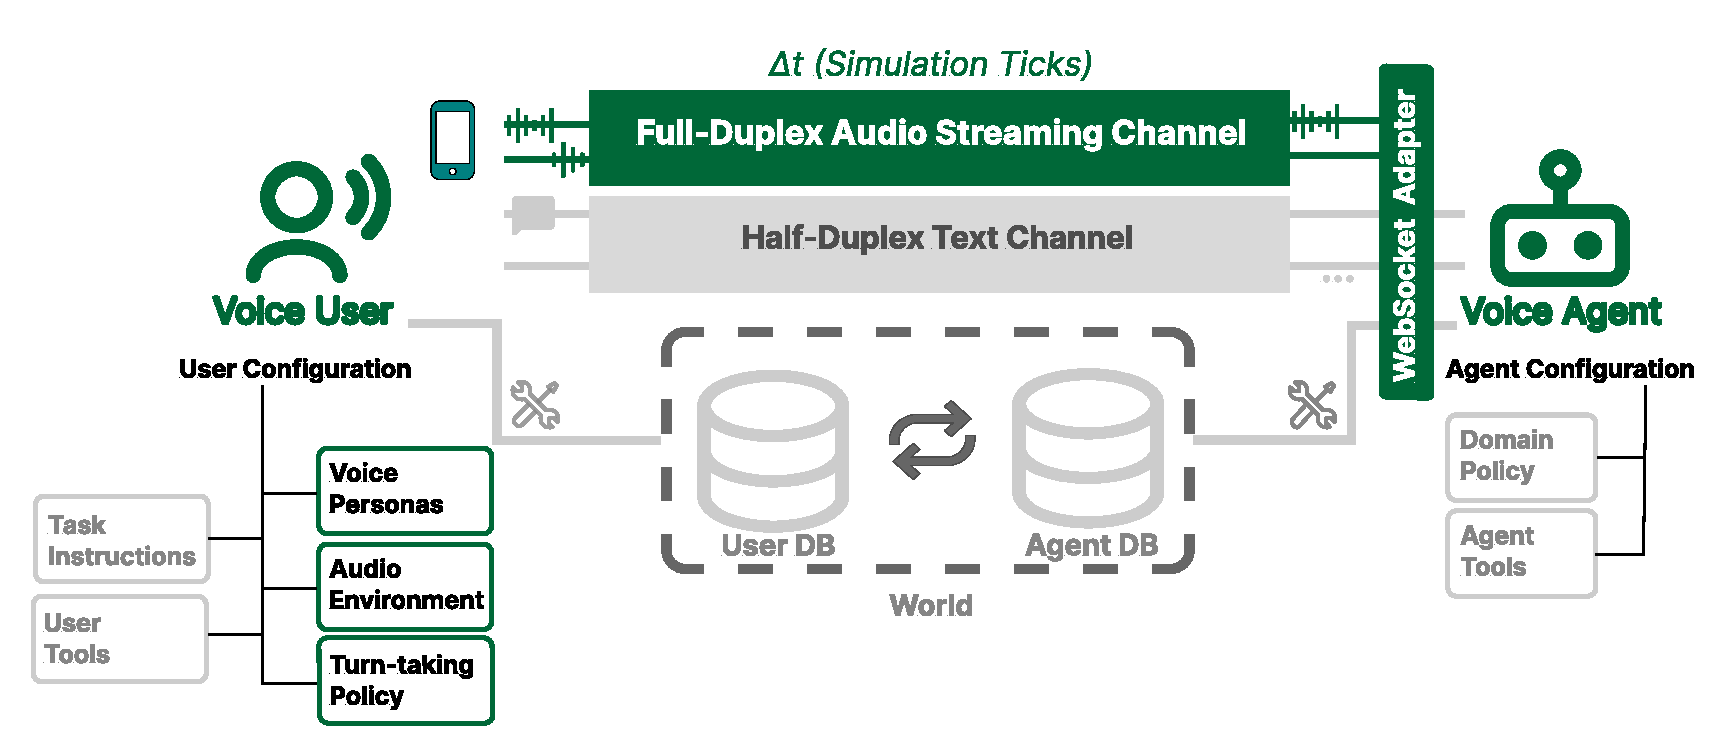
\includegraphics[width=\columnwidth]{figures/arch_diagram.pdf}
\caption{\tauvoice{} extends \tautwobench{} (gray) with voice-specific components (green): a voice user simulator with configurable personas, audio environment, and turn-taking policy; a full-duplex audio streaming channel discretized into simulation ticks; and a provider adapter for adding new voice APIs. Task infrastructure (instructions, tools, databases, domain policies) is inherited.}
\label{fig:architecture}
\end{figure}

The orchestrator coordinates the interaction loop between the voice user simulator and the agent API, managing audio exchange, turn-taking events, and evaluation logging. Voice agent APIs (OpenAI Realtime~\citep{openai_introducing_2025}, Gemini Live~\citep{vertex_ai_gemini_2025}, xAI Grok~\citep{xai_grok_voice_2025}) are designed for continuous real-time streaming with bidirectional audio flow and voice activity detection (VAD) for turn-taking. Crucially, these APIs index events on \textit{audio time} rather than wall-clock time---audio can be sent faster or slower than real-time and the API processes it according to audio timestamps.

This decoupling enables our tick-based orchestrator: by advancing simulation time independently of wall-clock time, we allow the user simulator to use the most capable LLM without real-time constraints, ensuring reliable instruction following and turn-taking decisions. This enables reproducibility and fine-grained control over the timing of all turn-taking actions.

\paragraph{Discrete Simulation Time.} We discretize the continuous audio stream into fixed-duration \textbf{ticks} ($\tau = 200$ms by default). Each tick, both parties exchange exactly $\tau$ ms of audio, enabling true full-duplex interaction where both can speak simultaneously. Since audio generation may not align with tick boundaries, both sides buffer; on interruption, the buffer is cleared, truncating the agent's in-progress response (formal details in Appendix~\ref{app:buffer-formalism}). The agent returns both audio and transcript text each tick, with text distributed proportionally to audio duration (Appendix~\ref{sec:proportional-text}); overlapping speech is linearized to sequential text for the user simulator LLM (Appendix~\ref{app:linearization}).

\paragraph{Controllability and Reproducibility.} Decoupling from real-time enables fine-grained control over all simulation parameters. Conversational dynamics are configurable: silence thresholds before responding, interruption check intervals, yield timing after overlap. The audio environment is fully parameterized: background noise SNR and drift, burst noise rate and intensity, telephony compression settings, and frame drop probability via a Gilbert-Elliott model. Voice personas specify accent, speaking style, and prosody. This enables systematic ablations isolating the impact of individual factors on task performance. Given a seed, all stochastic elements are deterministic for controlled comparison across agents; full reproducibility is limited only by LLM output variance.


\subsection{Voice User Simulator}
\label{sec:voice-user-simulator}

Voice interactions introduce challenges absent from text: the \textit{audio environment} degrades signals, and \textit{conversational dynamics} require real-time turn-taking decisions. Our simulator addresses these by generating realistic caller audio through a pipeline (Figure~\ref{fig:audio-pipeline}) combining text generation, speech synthesis, audio environment simulation, and conversational dynamics.

To isolate agent performance from transcription artifacts, the simulator receives the agent's transcript directly rather than transcribing agent speech.

\begin{figure}[ht]
\centering
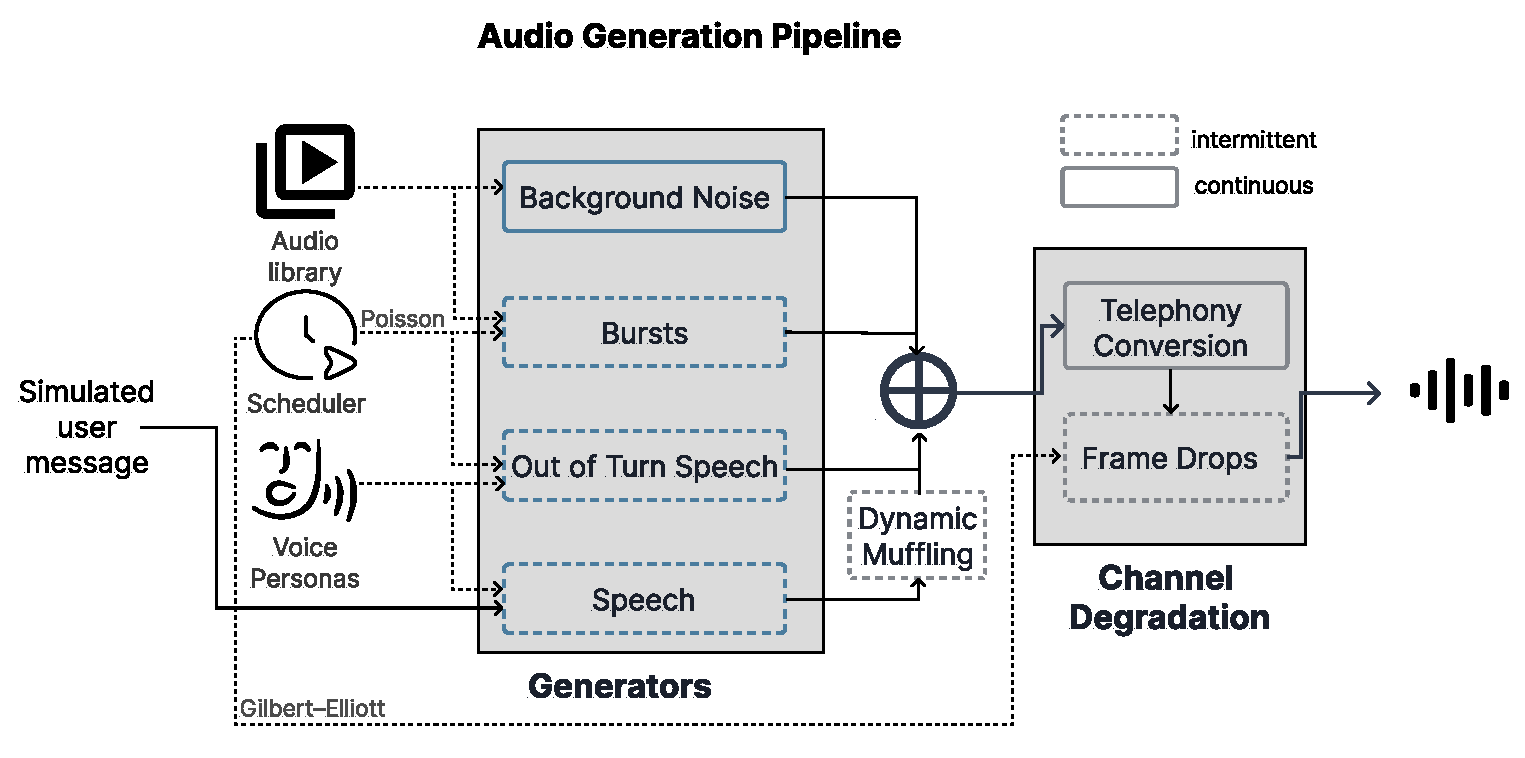
\includegraphics[width=\columnwidth]{figures/audio_pipeline.pdf}
\caption{Voice user simulator pipeline. Each tick, the simulator generates text, synthesizes speech with a persona, mixes in environmental audio, and applies telephony degradation to produce realistic caller audio.}
\label{fig:audio-pipeline}
\end{figure}

\paragraph{Speech Generation.} User simulator prompts produce natural spoken language: disfluencies and fillers (``um'', ``uh''), verbalized special characters (``at'' not ``@''), and terse responses. Generated text is synthesized using voice personas---each with a dedicated TTS voice and system prompt guiding speech style and prosody. We define seven personas spanning diverse accents and demographics (Appendix~\ref{app:personas}).

\paragraph{Audio Environment.} We simulate realistic telephony conditions by mixing synthesized speech with environmental audio: continuous background noise (chatter, traffic) and intermittent bursts (phone rings, dog barks) drawn from recorded samples. Out-of-turn speech---synthesized phrases like ``hold on'' and vocal tics like coughs and sneezes---simulates moments when callers are distracted. Effects degrade the signal: dynamic muffling simulates movement away from the microphone, telephony conversion applies G.711 $\mu$-law compression at 8kHz, and frame drops simulate packet loss. All streams are mixed to target signal-to-noise ratios relative to the primary speech. Parameters appear in Appendix~\ref{app:audio-effects}.

\paragraph{Turn-Taking Policy.} The simulator combines configurable threshold-based timing with LLM-driven decisions. For example, the user waits for a silence threshold (default 1s) before responding. During agent speech, an LLM periodically evaluates whether to interrupt based on conversation context. A separate LLM decides whether to backchannel (``mm-hmm''), and if the agent interrupts, the user yields after a configurable overlap duration. Full prompts appear in Appendix~\ref{app:turn-taking-prompts}; Table~\ref{tab:tick-example} illustrates these dynamics.


\subsection{Evaluation}

Voice evaluation requires capturing both task outcomes and conversational behavior. We instrument each simulation to log turn-taking events, audio effects, and agent responses, then derive metrics for task success and voice interaction quality.

\begin{table}[ht]
\caption{Key moments from the Task 41 trajectory (Figure~\ref{fig:speech-timeline}). At 8s, the agent interrupts; at 68s the user interrupts and the agent yields but fails to respond for 5 seconds; at 82s the agent incorrectly responds to non-agent-directed speech [in brackets]; at 113s the user interrupts but the agent does not yield; at 121s the agent correctly continues through a backchannel.}
\label{tab:tick-example}
\centering
\scriptsize
\resizebox{\columnwidth}{!}{%
\begin{tabular}{@{}rlll@{}}
\toprule
\textbf{Time} & \textbf{User} & \textbf{Agent} & \textbf{Event} \\
\midrule
5--8s & Hi, I have two prob- & & \\
8s & -lems. First, I ordered & Hello! & \textit{agent int.} \\
\addlinespace
\multicolumn{4}{c}{\ldots} \\
\addlinespace
60--67s & & ...Which would you like & \\
67--68s & & to do first? & \\
68--69s & Jigsaw first. & & \textit{user int., yield} \\
69--74s & & & \textit{no response} \\
74--77s & Can you switch it... & & \\
\addlinespace
\multicolumn{4}{c}{\ldots} \\
\addlinespace
77--82s & & To confirm, you want to & \\
82s & [Give me a moment.] & exchange the puzzle-- & \textit{non-dir., yield} \\
84s & & Sure, take your time. & \textit{error: responds} \\
\addlinespace
\multicolumn{4}{c}{\ldots} \\
\addlinespace
108--113s & & ...on order \#W4082615. Is & \\
113--114s & Yeah, that's it. & that the one? We can exch- & \textit{user int.} \\
114--115s & & -ange it for a puzzle... & \textit{no yield} \\
\addlinespace
\multicolumn{4}{c}{\ldots} \\
\addlinespace
115--121s & & ...500-piece puzzles. Wo- & \\
121--122s & mm-hmm & -uld you like to exchange & \textit{backchannel} \\
122--128s & & it for one of those? & \textit{continues} \\
\bottomrule
\end{tabular}%
}
\end{table}

\begin{figure*}[t]
\centering
\includegraphics[width=\textwidth]{figures/task_41_data/speech activity timeline.pdf}
\caption{Speech activity timeline from a Retail domain simulation with Gemini Live. A customer calls about exchanging a jigsaw puzzle and correcting their address. The legend distinguishes \textit{observations} (User Int.\ = user interruption, Non-Agent Dir.\ = speech to someone other than the agent, Burst = environmental burst noise) from \textit{evaluation markers} (Agent Int.\ = agent interruption, BC Issue = incorrect backchannel handling, Voc.\ Tic Error / Non-Agent Dir.\ Error = agent incorrectly yielding or responding to these stimuli).}
\label{fig:speech-timeline}
\end{figure*}

\paragraph{Timeline Walkthrough.}  Figure~\ref{fig:speech-timeline} illustrates our evaluation on a 3-minute Retail conversation with street noise. Key phenomena include: agent interruptions (red $\blacktriangle$) revealing turn-taking calibration; user interruptions where the agent yields but fails to respond (no-response error $\times$); non-agent-directed speech (pink \ldots) where the agent incorrectly yields; and backchannels (green $\circ$) correctly recognized as acknowledgment. Audio degradation (frame drops, muffling, burst noise) tests acoustic robustness throughout. This single example contains 8 user interruptions, 5 agent interruptions, 2 no-response errors, and 12 frame drops---illustrating the complexity our metrics capture (full transcript in Appendix~\ref{app:examples}).

\paragraph{Metrics.} We evaluate both \textit{task success} (pass@1, following \tautwobench{}: comparing final database state against annotated goals, plus verifying agent communications---for which we use LLM evaluation instead of string matching to handle spoken output variability) and \textit{voice interaction quality} across four dimensions: responsiveness, latency, interrupt rate, and selectivity. We also manually review a sample of failures to categorize error sources across the user and agent (\S\ref{sec:results}).



% Section 4: Experimental Setup
\section{Experimental Setup}
\label{sec:experiments}

\subsection{Domains and Tasks}

We evaluate on three domains from \tautwobench{}, totaling 278 tasks:
\begin{itemize}[nosep,leftmargin=*]
    \item \textbf{Retail} (114 tasks): Returns, exchanges, cancellations, and order modifications---often combined in a single conversation. Many tasks require handling ambiguous requests or customers who change their mind mid-conversation.
    \item \textbf{Airline} (50 tasks): Flight changes, cancellations, seat upgrades, and booking modifications requiring verification of passenger details and fare rules.
    \item \textbf{Telecom} (114 tasks): Plan changes, billing inquiries, service activations, and account modifications involving authentication and policy verification.
\end{itemize}
We designate \textbf{Retail as the primary evaluation domain} due to its heavy reliance on slot filling---collecting names, emails, order IDs, and addresses---where end-to-end speech systems are known to struggle~\citep{li_cb-whisper_2024, si_spokenwoz_2025}. Airline and Telecom serve as supporting domains to test generalization.

\subsection{Models}

We evaluate three audio-native providers, all released in the latter half of 2025:

\begin{table}[h]
\caption{Audio-native models evaluated.}
\label{tab:models}
\centering
\begin{small}
\resizebox{\columnwidth}{!}{%
\begin{tabular}{llll}
\toprule
\textbf{Provider} & \textbf{Model} & \textbf{Protocol} & \textbf{Release} \\
\midrule
OpenAI & \texttt{gpt-realtime-2025-08-28} & WebSocket & Aug 2025 \\
Google & \texttt{gemini-live-2.5-flash} & WebSocket & Dec 2025 \\
xAI & \texttt{grok-voice-agent} & WebSocket & Dec 2025 \\
\bottomrule
\end{tabular}%
}
\end{small}
\end{table}

All models receive identical system prompts with voice-specific guidance: when collecting names, emails, or IDs, ask customers to spell letter-by-letter; if authentication fails, explicitly request spelling again.

\subsection{Evaluation Conditions}

We evaluate each provider under two speech complexity conditions:

\begin{table}[h]
\caption{Speech complexity conditions: Clean vs Realistic.}
\label{tab:conditions}
\centering
\begin{small}
\resizebox{\columnwidth}{!}{%
\begin{tabular}{@{}llll@{}}
\toprule
\textbf{Category} & \textbf{Setting} & \textbf{Clean} & \textbf{Realistic} \\
\midrule
\multirow{1}{*}{Accents} & Personas & American & Diverse accents \\
\midrule
\multirow{5}{*}{Audio/Channel} & Background noise & None & Indoor/outdoor \\
 & Burst noise & None & $\sim$1/min \\
 & Frame drops & None & $\sim$2.0\% (G-E model) \\
 & Telephony & G.711 $\mu$-law 8kHz & G.711 $\mu$-law 8kHz \\
 & Muffling & None & Dynamic \\
\midrule
\multirow{4}{*}{User Behavior} & Involuntary sounds & None & Coughs, sneezes \\
 & Non agent-directed speech & None & ``hold on'', ``one sec'' \\
 & Interruptions & None & LLM-based \\
 & Backchanneling & None & LLM-based \\
\bottomrule
\end{tabular}%
}
\end{small}
\end{table}

\textbf{Clean} simulates an idealized telephony scenario: clear American-accented speech with no background noise or user interruptions. \textbf{Realistic} reflects realistic phone interactions: diverse speaker accents, environmental noise (indoor/outdoor backgrounds, burst sounds), channel degradation (frame drops, muffling), and natural user behaviors (interruptions, backchanneling, vocal tics, non-directed speech). To isolate the contribution of each factor, we also evaluate intermediate ablation conditions adding noise, accents, or user behaviors independently (Table~\ref{tab:conditions-ablation-single}).

\begin{table}[h]
\caption{Speech complexity conditions by ablation (single factors). Columns: Cln=Clean, +N=Noise, +A=Accents, +I=Interrupts, Real=Realistic (all effects).}
\label{tab:conditions-ablation-single}
\centering
\begin{small}
\resizebox{\columnwidth}{!}{%
\begin{tabular}{llccccc}
\toprule
\textbf{Category} & \textbf{Setting} & \textbf{Cln} & \textbf{+N} & \textbf{+A} & \textbf{+I} & \textbf{Real} \\
\midrule
\multirow{1}{*}{Accents} & Personas &  &  & \checkmark &  & \checkmark \\
\midrule
\multirow{5}{*}{Audio/Channel} & Background noise &  & \checkmark &  &  & \checkmark \\
 & Burst noise &  & \checkmark &  &  & \checkmark \\
 & Frame drops &  & \checkmark &  &  & \checkmark \\
 & Telephony & \checkmark & \checkmark & \checkmark & \checkmark & \checkmark \\
 & Muffling &  & \checkmark &  &  & \checkmark \\
\midrule
\multirow{4}{*}{User Behavior} & Involuntary sounds &  &  &  & \checkmark & \checkmark \\
 & Non agent-directed speech &  &  &  & \checkmark & \checkmark \\
 & Interruptions &  &  &  & \checkmark & \checkmark \\
 & Backchanneling &  &  &  & \checkmark & \checkmark \\
\bottomrule
\end{tabular}%
}
\end{small}
\end{table}

This 3$\times$3$\times$2 design (3 providers $\times$ 3 domains $\times$ 2 conditions) isolates the impact of acoustic realism on task completion. Ablation conditions are evaluated on the Retail domain to identify which factors contribute most to performance degradation.

\subsection{Simulation Parameters}

Each task runs with a fixed seed for reproducible effect scheduling (noise timing, frame drops), though LLM responses remain non-deterministic. Reproducibility refers to controlled inputs and deterministic non-LLM components; stochasticity arises from agent and simulator LLMs. Key parameters: tick duration 200ms, max conversation 1200s, user simulator LLM GPT-4.1, TTS via ElevenLabs v3 at 24kHz, interruption and backchannel check every 2s.

\subsection{Metrics}

\textbf{Task Completion:} Following \tautwobench{}, tasks are fully verifiable: success is deterministically evaluated by comparing the end state of the environment (e.g., database records) against a gold standard. We report pass@1---the proportion of tasks completed successfully on a single attempt.

\textbf{Voice Interaction Quality:} Beyond task completion, we evaluate how well agents manage real-time conversation. Effective turn-taking requires \textit{responsiveness} (acting when action is needed), \textit{latency} (reacting quickly), \textit{not interrupting} (good timing), and \textit{selectivity} (ignoring backchannels and non-directed speech). We measure:
\begin{itemize}[nosep,leftmargin=*]
    \item \textbf{Responsiveness:} Response Rate ($R_R$, proportion of user turns receiving a response) and Yield Rate ($R_Y$, proportion of interruptions where agent yields within 2s).
    \item \textbf{Latency:} Response Latency ($L_R$, time from user utterance end to agent response) and Yield Latency ($L_Y$, time to stop speaking after interruption).
    \item \textbf{Interrupt:} Agent Interruption Rate ($I_A$, proportion of turns where agent speaks before user finishes; $>$100\% means multiple interruptions per turn).
    \item \textbf{Selectivity:} Correctly ignoring backchannels ($S_{BC}$), vocal tics ($S_{VT}$), and non-directed speech ($S_{ND}$).
\end{itemize}
We report four aggregate scores: \textbf{Responsiveness} $= \mathrm{avg}(R_R, R_Y)$, \textbf{Latency} $= \mathrm{avg}(L_R, L_Y)$, \textbf{Interrupt} $= I_A$, and \textbf{Selectivity} $= \mathrm{avg}(S_{BC}, S_{VT}, S_{ND})$. See Appendix~\ref{app:voice-metrics} for detailed definitions.


% Section 5: Results
\section{Results}
\label{sec:results}

\subsection{Quantitative Results}

\subsubsection{Task Completion}

Figure~\ref{fig:headline} and Table~\ref{tab:text-control-regular} present our headline finding: \textbf{voice agents show substantial drops from text baselines}. Under \textbf{Clean} conditions (studio-quality audio, American accents), the best voice provider already drops 38pp from GPT-5 (42\% vs GPT-5 at 80\%). Under \textbf{Realistic} conditions (background noise, diverse accents, natural user behaviors), performance drops an additional 12pp to 30\%. This gap persists even against non-reasoning text models: compared to GPT-4.1 (54\%), voice still drops 12pp (Clean) to 24pp (Realistic).

\begin{table}[h]
\caption{Text vs Voice comparison (pass@1). Text shows GPT-5 (reasoning) and GPT-4.1 (non-reasoning). Voice evaluated under Clean and Realistic conditions. Deltas show gap from GPT-5.}
\label{tab:text-control-regular}
\centering
\begin{small}
\resizebox{\columnwidth}{!}{%
\begin{tabular}{@{}llccc@{}}
\toprule
 &  &  & \multicolumn{2}{c}{\textbf{Voice}} \\
\cmidrule(l){4-5}
\textbf{Domain} & \textbf{Provider} & \textbf{Text} & \textbf{Clean} & \textbf{Realistic} \\
\midrule
\multirow{3}{*}{All} & Google & \multirow{3}{*}{79\% (54\%)} & 29\% (-50) & 24\% (-55) \\
 & OpenAI &  & 33\% (-46) & 19\% (-60) \\
 & xAI &  & \textbf{42\% (-37)} & \textbf{30\% (-49)} \\
\midrule
\multirow{3}{*}{Retail} & Google & \multirow{3}{*}{81\% (74\%)} & 39\% (-42) & \textbf{28\% (-53)} \\
 & OpenAI &  & 39\% (-42) & 15\% (-65) \\
 & xAI &  & \textbf{42\% (-39)} & 20\% (-61) \\
\midrule
\multirow{3}{*}{Airline} & Google & \multirow{3}{*}{62\% (56\%)} & 28\% (-34) & 26\% (-36) \\
 & OpenAI &  & \textbf{36\% (-26)} & 28\% (-34) \\
 & xAI &  & 26\% (-36) & \textbf{34\% (-28)} \\
\midrule
\multirow{3}{*}{Telecom} & Google & \multirow{3}{*}{95\% (34\%)} & 20\% (-75) & 19\% (-76) \\
 & OpenAI &  & 23\% (-72) & 14\% (-81) \\
 & xAI &  & \textbf{58\% (-37)} & \textbf{36\% (-59)} \\
\bottomrule
\multicolumn{5}{l}{\footnotesize \textit{Text column: GPT-5, reasoning (GPT-4.1, best non-reasoning model). Deltas relative to GPT-5.}} \\
\end{tabular}
}
\end{small}
\end{table}

The 12pp drop from Clean to Realistic conditions accounts for roughly one-quarter of the total voice-text gap; the remaining three-quarters reflects the drop from text to Clean voice.

Across providers, \textbf{xAI achieves the highest scores} (42\% Clean, 30\% Realistic), while \textbf{Google shows the smallest degradation} under realistic conditions ($-$5pp vs $-$12--14pp for others). Domain-specific patterns emerge: xAI substantially outperforms others in Telecom (59\% Clean vs 20--24\% for others), while performance is more similar across providers in Retail and Airline.

\paragraph{Statistical Reliability.} For Retail, where we conducted 3 independent runs per condition, both the text-to-Clean gap and the Clean-to-Realistic gap are statistically significant (non-overlapping 95\% CIs). Voice providers achieve 36--39\% $\pm$ 3--6pp (Clean) and 12--26\% $\pm$ 2--4pp (Realistic), compared to text baselines of 73\% $\pm$ 3pp (GPT-4.1) and 82\% $\pm$ 1pp (GPT-5). Full statistical breakdown in Appendix~\ref{app:stat-sig}.

\subsubsection{Impact of Acoustic Realism}

To isolate which factors hurt performance most, we conduct ablations on the Retail domain, adding noise, accents, or user behaviors independently (Table~\ref{tab:ablation-single}).

\begin{table}[h]
\caption{Ablation: impact of individual acoustic factors on pass@1 (Retail domain).}
\label{tab:ablation-single}
\centering
\begin{small}
\resizebox{\columnwidth}{!}{%
\begin{tabular}{lccc|c}
\toprule
\textbf{Condition} & \textbf{Google} & \textbf{OpenAI} & \textbf{xAI} & \textbf{All} \\
\midrule
Clean & 39\% & 39\% & \textbf{42\%} & 40\% \\
+ Noise & \textbf{37\% (-1)} & 26\% (-13) & 29\% (-12) & 31\% (-9) \\
+ Accents & \textbf{36\% (-2)} & 21\% (-18) & 23\% (-18) & 27\% (-13) \\
+ Interrupts & \textbf{38\% (+0)} & 30\% (-8) & 36\% (-5) & 35\% (-4) \\
Realistic & \textbf{28\% (-11)} & 15\% (-23) & 20\% (-21) & 21\% (-19) \\
\bottomrule
\end{tabular}%
}
\end{small}
\end{table}

\textbf{Accents are the most damaging factor}, causing a 13pp average drop (vs 9pp for noise, 5pp for interrupts). This finding has accessibility implications: users with non-American accents may face systematically worse service. OpenAI and xAI are particularly vulnerable to accents ($-$18pp each), while Google shows greater robustness ($-$2pp). Because accents are implemented via TTS personas, these results should be interpreted as indicative rather than definitive.

\textbf{Google is consistently the most robust provider} across individual ablation conditions, with minimal degradation from noise ($-$2pp) or interrupts ($-$1pp). However, Google's robustness to isolated factors does not fully transfer to compound stress: individual effects sum to just $-$5pp, yet the full Realistic condition causes $-$11pp---suggesting super-additive interactions when multiple factors combine. This 11pp drop still compares favorably to 22--24pp for competitors.

\subsubsection{Voice Interaction Quality}

Beyond task completion, we evaluate conversational dynamics under Realistic conditions (Table~\ref{tab:voice-quality}). We report four aggregate dimensions: \textbf{Latency} (how quickly agents react), \textbf{Responsiveness} (whether agents act when needed), \textbf{Interrupt} (how often agents cut off users mid-speech), and \textbf{Selectivity} (whether agents correctly ignore signals that do not require action).

\begin{table}[h]
\caption{Voice interaction quality (Realistic condition, aggregated across domains). \textbf{Bold} indicates best. Full breakdown in Appendix~\ref{app:voice-metrics-detail}.}
\label{tab:voice-quality}
\centering
\begin{small}
\resizebox{\columnwidth}{!}{%
\begin{tabular}{@{}lcccc@{}}
\toprule
\textbf{Provider} & \textbf{Latency}$\downarrow$ & \textbf{Responsiveness}$\uparrow$ & \textbf{Interrupt}$\downarrow$ & \textbf{Selectivity}$\uparrow$ \\
\midrule
Google & 1.13s & 71\% & \textbf{24\%} & 51\% \\
OpenAI & 2.22s & 68\% & 34\% & \textbf{74\%} \\
xAI & \textbf{0.99s} & \textbf{85\%} & 104\% & 51\% \\
\bottomrule
\end{tabular}
}
\end{small}
\end{table}

\textbf{xAI achieves the best latency and responsiveness}: fastest reactions (0.99s average latency) and highest responsiveness (85\%). However, this speed comes at a severe cost: xAI has an interrupt rate of 104\%---interrupting users more than once per turn on average.

\textbf{OpenAI shows the opposite trade-off}: slowest latency (2.22s) and lowest responsiveness (68\%), but highest selectivity (74\%) and a moderate interrupt rate (34\%). OpenAI is more conservative, waiting longer to ensure genuine user intent before responding.

\textbf{Google achieves the best balance}: lowest interrupt rate (24\%), reasonable latency (1.13s), and mid-range selectivity (51\%), though with lower responsiveness (71\%). No provider achieves both high responsiveness and low interruption, highlighting the fundamental challenge of real-time turn-taking.

\subsection{Qualitative Error Analysis}
\label{sec:analysis}

To characterize failure modes beyond aggregate pass rates---and to verify that observed failures stem from agent behavior rather than artifacts of the benchmark or user simulator---we perform a qualitative error analysis.

\paragraph{Task Selection.} We define $\text{pass}_{\text{text}}$ as tasks where both GPT-4.1 and GPT-5.2 (medium reasoning) succeed in text mode, $\text{pass}_{\text{clean}}$ as tasks where a majority of audio providers succeed under Clean conditions, and $\text{pass}_{\text{realistic}}$ as tasks where a majority succeed under Realistic conditions. We construct two analysis cohorts:
\begin{itemize}[nosep,leftmargin=*]
    \item \textbf{Voice-Fragile}: Tasks that satisfy $\text{pass}_{\text{text}}$ but not $\text{pass}_{\text{clean}}$, isolating inherent voice interaction challenges.
    \item \textbf{Noise-Fragile}: Tasks that satisfy $\text{pass}_{\text{clean}}$ but not $\text{pass}_{\text{realistic}}$, isolating the impact of acoustic realism (noise, accents, interruptions).
\end{itemize}
For each cohort, we sample 20 tasks, prioritizing those exhibiting the largest performance gap between conditions. For each sampled task, we randomly select one failing provider for analysis.

\paragraph{Annotation Procedure.} Two independent raters examined each failed simulation, labeling: (1) \textit{error source}---whether the agent or user simulator caused the first critical error; and (2) \textit{error type}---one of logical, transcription, VAD/unresponsive, hallucination, or early termination. Inter-rater agreement was 92.5\% (37/40 tasks); disagreements were resolved through discussion.

\paragraph{Results.} Table~\ref{tab:combined-error-analysis} shows the distribution of error types by source for both cohorts. Full annotations are in Appendix~\ref{app:qualitative-analysis}.

\begin{table}[h]
\caption{Error analysis: distribution of error types by source. Agent errors dominate in both cohorts (75\% and 90\%).}
\label{tab:combined-error-analysis}
\centering
\begin{small}
\resizebox{0.85\columnwidth}{!}{%
\begin{tabular}{@{}llcc@{}}
\toprule
\textbf{Source} & \textbf{Error Type} & \makecell{\textbf{Voice-}\\\textbf{Fragile}} & \makecell{\textbf{Noise-}\\\textbf{Fragile}} \\
\midrule
\multirow{5}{*}{Agent} & Logical & 8 & 6 \\
& Transcription & 4 & 4 \\
& VAD & 2 & 1 \\
& Unresponsive & 1 & 7 \\
\cmidrule{2-4}
& \textit{Total} & \textit{15 (75\%)} & \textit{18 (90\%)} \\
\midrule
\multirow{4}{*}{User} & Logical & 1 & 1 \\
& Hallucination & 3 & 1 \\
& Early Term. & 1 & -- \\
\cmidrule{2-4}
& \textit{Total} & \textit{5 (25\%)} & \textit{2 (10\%)} \\
\bottomrule
\end{tabular}
}
\end{small}
\end{table}

\textbf{Agent errors dominate}: 75\% of failures in the Voice-Fragile cohort and 90\% in the Noise-Fragile cohort are attributed to the agent rather than the user simulator---suggesting that observed failures primarily reflect agent behavior under our evaluation setup, not simulator artifacts.

\textbf{Logical errors are most common in the Voice-Fragile cohort} (8/20), indicating that voice agents struggle with reasoning even when transcription is accurate. However, \textbf{VAD/unresponsive errors become dominant in the Noise-Fragile cohort} (8/20), where background noise and interruptions cause agents to miss user utterances or become unresponsive.


% Section 6: Conclusion
\section{Conclusion}
\label{sec:conclusion}

\subsection{Limitations}

\textbf{Language and Speech:} We evaluate English only using TTS rather than recorded speech. Since TTS is more enunciated than real callers, our setup represents a lower bar for voice systems. Accent findings via TTS personas should be interpreted as indicative rather than definitive.

\textbf{Evaluation Scope:} We measure task completion and conversational dynamics, but not agent speech generation quality (tone, naturalness), user satisfaction, or partial task success.

\textbf{Simulator Fidelity:} Our simulator is more patient than real users, with perfect memory and instantaneous tool calls. We decouple from wall-clock time for controllability, but validated this choice by testing with artificial 5-second response delays---observing no adverse effects on agent behavior. In practice, the p95 simulator processing time is $\sim$1.5 seconds, well within conversational tolerance.

\textbf{Transcript Injection:} The simulator bypasses ASR on the agent side by feeding transcripts directly to the user simulator LLM. In our error analysis (Section~\ref{sec:analysis}), annotators found agent speech intelligible in 100\% of the 40 sampled tasks, suggesting this simplification has minimal impact.

\subsection{Future Work}

Future directions include tool call latency, agent speech quality evaluation, non-English languages, and human user studies to validate simulator dynamics. Adding cascaded ASR$\rightarrow$LLM$\rightarrow$TTS baselines (supported by \tauvoice{}'s architecture) would help isolate voice modality effects from architecture choices. 

\subsection{Conclusion}

We introduced \textbf{\tauvoice{}}, extending \tautwobench{} to full-duplex voice with 278 tasks across retail, airline, and telecom domains. Our evaluation reveals a substantial voice-text gap: while GPT-5 (reasoning) achieves 80\%, voice agents reach only 29--42\% under clean conditions and 19--30\% under realistic conditions---a 50--61pp gap. Error analysis attributes 75--90\% of failures to agent behavior rather than simulator artifacts, suggesting the benchmark measures genuine agent limitations. We release \tauvoice{} to support development of voice agents that reliably complete tasks under realistic conditions.
% 

%%%%%%%%%%%%%%%%%%%%%%%%%%%%%%%%%%%%%%%%%%%%%%%%%%%%%%%%%%%%%%%%%%%%%%%%%%%%%%%
% ACKNOWLEDGEMENTS & IMPACT STATEMENT (unnumbered, before references)
%%%%%%%%%%%%%%%%%%%%%%%%%%%%%%%%%%%%%%%%%%%%%%%%%%%%%%%%%%%%%%%%%%%%%%%%%%%%%%%

% Acknowledgements should only appear in the accepted version.
% Comment out during initial submission for blind review.
% \section*{Acknowledgements}

% NOTE: Do NOT include acknowledgements in the initial blind submission.
% Only add for camera-ready version after acceptance.
%
% Typically includes thanks to:
% - Reviewers who gave useful comments
% - Colleagues who contributed to ideas
% - Funding agencies and corporate sponsors

% TODO: Write acknowledgements here (for camera-ready only)



% Impact Statement (REQUIRED for ICML 2026)
\section*{Impact Statement}

% REQUIRED for ICML 2026: Statement of the potential broader impact of your work,
% including ethical aspects and future societal consequences.
% This section does not count toward the page limit.

\textbf{Accessibility.} Our ablation results show performance degradation with diverse accents, raising equity concerns: voice agents risk excluding users who might benefit most from voice interfaces. Evaluating under realistic conditions helps identify these gaps.

\textbf{Open and extensible.} We open-source \tauvoice{} as a fully configurable platform. Researchers can bring their own TTS, STT, voice agents, cascaded models and VAD implementations. All parameters are configurable: audio effects, voice personas, turn-taking policies, and the user simulator LLM. This modularity enables evaluation of new providers, languages, and domains without rebuilding infrastructure.

\textbf{Our position.} Transparent benchmarking under realistic conditions helps the community understand deployment readiness. Measuring where voice agents fail is a prerequisite for improving them.


%%%%%%%%%%%%%%%%%%%%%%%%%%%%%%%%%%%%%%%%%%%%%%%%%%%%%%%%%%%%%%%%%%%%%%%%%%%%%%%
% REFERENCES
%%%%%%%%%%%%%%%%%%%%%%%%%%%%%%%%%%%%%%%%%%%%%%%%%%%%%%%%%%%%%%%%%%%%%%%%%%%%%%%
\bibliography{tau-voice}
\bibliographystyle{icml2026}

%%%%%%%%%%%%%%%%%%%%%%%%%%%%%%%%%%%%%%%%%%%%%%%%%%%%%%%%%%%%%%%%%%%%%%%%%%%%%%%
% APPENDIX (optional, no page limit)
%%%%%%%%%%%%%%%%%%%%%%%%%%%%%%%%%%%%%%%%%%%%%%%%%%%%%%%%%%%%%%%%%%%%%%%%%%%%%%%
\newpage
\appendix
\onecolumn
% Appendix: No page limit, but keep focused and relevant.

\section*{Appendix Overview}
This appendix provides implementation details for reproducibility:
\begin{itemize}
    \item \textbf{Appendix A}: Hyperparameter settings
    \item \textbf{Appendix B}: Full-duplex audio processing (buffer formalism, text distribution, linearization)
    \item \textbf{Appendix C--F}: Voice simulation configuration (personas, audio effects, turn-taking prompts, system prompts)
    \item \textbf{Appendix G}: Additional experimental results
    \item \textbf{Appendix H}: Complete example conversation with annotations
\end{itemize}

% A. Experimental Setup
\section{Simulation Parameters}
\label{app:hyperparams}

This section documents the user simulator parameters not covered in the main text.

\subsection{Turn-Taking Thresholds}

Table~\ref{tab:turn-taking-thresholds} shows the turn-taking thresholds.

\begin{table}[h]
\centering
\small
\begin{tabular}{lrl}
\toprule
\textbf{Parameter} & \textbf{Default} & \textbf{Description} \\
\midrule
Wait-to-respond (other) & 1.0s & Min silence from agent before user responds \\
Wait-to-respond (self) & 5.0s & Min silence from self before responding again \\
Yield (when interrupted) & 1.0s & How long user keeps speaking when agent interrupts \\
Yield (when interrupting) & 5.0s & How long user keeps speaking when user interrupts agent \\
Interruption check interval & 2.0s & Interval for LLM interruption checks \\
Backchannel check interval & 2.0s & Interval for LLM backchannel checks \\
\bottomrule
\end{tabular}
\caption{Turn-taking thresholds controlling conversation flow.}
\label{tab:turn-taking-thresholds}
\end{table}

\paragraph{Backchanneling.} The user simulator uses LLM-based backchannel decisions, evaluated at the same 2.0s interval as interruption checks. The LLM determines whether to emit a backchannel (e.g., ``mm-hmm'', ``uh-huh'') based on conversation context.



% B. Orchestrator Implementation Details
\section{Full-Duplex Audio Processing}
\label{app:audio-processing}

\subsection{Buffer Formalism}
\label{app:buffer-formalism}

Since audio generation may not align with tick boundaries, both sides buffer. We formalize the agent-side buffer, where interruption semantics matter:
\begin{align}
a^t &= (B^{t-1} \oplus \tilde{a}^t)[0:\tau] \label{eq:agent-output}\\
B^t &= \begin{cases}
\emptyset & \text{if interrupted} \\
(B^{t-1} \oplus \tilde{a}^t)[\tau:] & \text{otherwise}
\end{cases} \label{eq:buffer-update}
\end{align}
where $\tilde{a}^t$ is the audio streamed by the API during tick $t$'s wall-clock duration, $B^t$ is the output buffer, and $\oplus$ denotes concatenation. On interruption, the buffer is cleared, truncating the agent's in-progress response.

\subsection{Proportional Text Distribution}
\label{sec:proportional-text}

Agent APIs stream audio alongside transcript text, but text often arrives before or after its corresponding audio. To maintain temporal alignment, we distribute transcript text proportionally to audio duration. For each utterance, let $T$ be the total transcript and $A_\text{total}$ the total audio bytes received. At each tick, we emit:
\[
T^t = T\left[0 : \frac{A_\text{played}^t}{A_\text{total}} \cdot |T|\right]
\]
where $A_\text{played}^t$ is the cumulative audio played through tick $t$. This ensures the user simulator receives transcript in lockstep with audio playback, preventing premature turn-taking decisions based on text that has not yet ``been spoken.''

\subsection{Linearization Algorithm}
\label{app:linearization}

Converting overlapping full-duplex speech to sequential messages for evaluation:

\textbf{Rule:} ``If you speak entirely during someone else's turn, you get inserted where you stopped. Otherwise, whoever started first goes first.''

Table~\ref{tab:linearization-rules} shows the handling for each overlap case.

\begin{table}[h]
\centering
\begin{tabular}{lll}
\toprule
\textbf{Case} & \textbf{Condition} & \textbf{Action} \\
\midrule
No overlap & Segments don't touch & Chronological order \\
Partial overlap & Segments cross, neither contained & Order by start time \\
Containment & X fully inside Y & Split Y at X's end, insert X there \\
\bottomrule
\end{tabular}
\caption{Linearization rules for converting overlapping speech to sequential messages.}
\label{tab:linearization-rules}
\end{table}


% C. Voice Simulation Configuration
\section{Voice Personas}
\label{app:personas}

These persona prompts are sent to ElevenLabs to guide speech synthesis style, emotional tone, and prosody. Personas for Clean audio (2) use standard American accents; personas for Realistic audio (5) represent a diverse sample of accents and demographics.

\subsection{Personas for Clean Audio}

\subsubsection{Matt Delaney}
\begin{quote}
\small
You are a middle-aged white man from the American Midwest. You always behave as if you are speaking out loud in a real-time conversation with a customer service agent. You are calm, clear, and respectful---but also human. You sound like someone who's trying to be helpful and polite, even when you're slightly frustrated or in a hurry. You value efficiency but never sound robotic.

You sometimes use contractions, informal phrasing, or small filler phrases (``yeah,'' ``okay,'' ``honestly,'' ``no worries'') to keep things natural. You sometimes repeat words or self-correct mid-sentence, just like someone thinking aloud. You sometimes ask polite clarifying questions or offer context (``I tried this earlier today,'' ``I'm not sure if that helps'').

You rarely use formal or stiff language (``considerable,'' ``retrieve,'' ``representative''). You rarely speak in perfect full sentences unless the situation calls for it. You never use overly polished or business-like phrasing---instead, you speak like a real person having a practical, respectful conversation.
\end{quote}

\subsubsection{Lisa Brenner}
\begin{quote}
\small
You are a white woman in your late 40s from a suburban area. You always speak as if you are talking out loud to a customer service agent who is already wasting your time. You're not openly hostile (yet), but you are tense, impatient, and clearly annoyed. You act like this issue should have been resolved the first time, and the fact that you're following up is unacceptable.

You often sound clipped, exasperated, or sarcastically polite. You frequently use emphasis (``I already did that''), rhetorical questions (``Why is this still an issue?''), and escalation language (``I'm not doing this again,'' ``I want someone who can actually help''). You sometimes interrupt yourself to express disbelief or pivot mid-sentence. You expect fast results and get irritated when things are repeated.

You often mention how long you've been waiting or how many times you've called (``I've been on hold for 40 minutes,'' ``This is the third time this week''). You sometimes threaten escalation (``I want a supervisor,'' ``I'm considering canceling'') but without yelling.

You never sound relaxed. You never use slow, reflective speech. You never thank the agent unless something gets resolved.
\end{quote}

\subsection{Personas for Realistic Audio}

\subsubsection{Mildred Kaplan}
\begin{quote}
\small
You are an elderly white woman in your early 80s calling customer service for help with something your grandson or neighbor usually does.
\end{quote}

\subsubsection{Arjun Roy}
\begin{quote}
\small
A Bengali man from Dhaka, Bangladesh in his mid-30s calling customer service about a billing issue. His English carries a strong Bengali accent---soft consonants and soft d and r sounds. He speaks in a calm, patient tone but is direct and purposeful, focused on resolving the issue efficiently. His pacing is slow, distracted with a warm yet firm timbre. The speech sounds like it is coming from far away.
\end{quote}

\subsubsection{Wei Lin}
\begin{quote}
\small
A Chinese woman in her late 20s from Sichuan, calling customer service about a credit card billing issue. She speaks English with a thick Sichuan Mandarin accent. She sounds upbeat, matter-of-fact, and distracted. Her tone is firm but polite, with fast pacing and smooth timbre. ok audio quality.
\end{quote}

\subsubsection{Mamadou Diallo}
\begin{quote}
\small
A Senegalese man who's first language is french in his mid-30s calling customer service about a billing issue. He speaks English with a strong French accent. His tone is hurried, slightly annoyed, and matter-of-fact, as if he's been transferred between agents and just wants the problem fixed.
\end{quote}

\subsubsection{Priya Patil}
\begin{quote}
\small
A woman in her early 30s from Maharashtra, India, calling customer support from her mobile phone. She speaks Indian English with a strong Maharashtrian accent---noticeable regional intonation and rhythm. Her tone is slightly annoyed and hurried, matter-of-fact, and focused on getting the issue resolved quickly. Her voice has medium pitch, firm delivery, short sentences, and faint background room tone typical of a phone call.
\end{quote}

\section{Audio Effects Configuration}
\label{app:audio-effects}

This section details the audio effects applied to user speech in the Realistic complexity preset (Section~\ref{sec:experiments}). These effects are demonstrated in the example conversation (Appendix~\ref{app:example-transcript}), which includes frame drops, burst noise, muffling, and non-directed speech events.

\subsection{Environment Presets}

Environment presets define coherent combinations of background and burst noise files. One background noise file is selected per task; all burst noise files for the environment are available. Table~\ref{tab:environment-presets} shows the available environments.

\begin{table}[h]
\centering
\begin{tabular}{lll}
\toprule
\textbf{Environment} & \textbf{Background Noise} & \textbf{Burst Noise} \\
\midrule
Indoor & People Talking, TV News & Ringing Phone, Dog Bark \\
Outdoor & Busy Street, Street \& Metro & Car Horn, Engine Idling, Siren \\
\bottomrule
\end{tabular}
\caption{Environment presets define which audio files are used for background and burst noise generation.}
\label{tab:environment-presets}
\end{table}

\subsection{Effect Scheduling}

Table~\ref{tab:effect-scheduling} shows the scheduling parameters for each audio effect type.

\begin{table}[h]
\centering
\begin{tabular}{lll}
\toprule
\textbf{Effect} & \textbf{Scheduling} & \textbf{Rate (Realistic Preset)} \\
\midrule
Burst noise & Poisson process & 1.0 events/min \\
Out-of-turn speech (phrases, vocal tics) & Poisson process & 0.7 events/min \\
Frame drops & Gilbert-Elliott model & 2\% avg loss rate, 100ms burst \\
Dynamic muffling & Per-utterance probability & 20\% of utterances \\
\bottomrule
\end{tabular}
\caption{Effect scheduling parameters for the Realistic complexity preset.}
\label{tab:effect-scheduling}
\end{table}

\paragraph{Out-of-Turn Speech.} Includes both non-directed phrases (e.g., ``Hold on a second,'' ``I'm on the phone,'' ``Give me a moment'') and vocal tics (coughs, sneezes, sniffles). These test the agent's ability to distinguish speech directed at it from background sounds.

\subsection{Gilbert-Elliott Model for Frame Drops}

Two-state Markov model for realistic bursty packet loss:
\begin{itemize}
    \item \textbf{Good state}: No packet loss ($k=0$)
    \item \textbf{Bad state}: 20\% loss probability ($h=0.2$)
    \item Transition rates derived from target loss rate and average burst duration
    \item Each frame drop event removes 150ms of audio
\end{itemize}

\subsection{Audio Mixing}

All audio streams are mixed using SNR-based normalization:
\begin{itemize}
    \item Background noise: 15 dB SNR (with $\pm$3 dB drift)
    \item Burst noise: sampled from $-5$ to $+10$ dB SNR per event
\end{itemize}

\section{Voice Interaction Metrics}
\label{app:voice-metrics}

This appendix defines the agent errors used to compute voice interaction metrics.

\paragraph{Timing thresholds.} Yield window: 2.0s (agent must stop within this time after user interruption). Selectivity windows: 1.0s for incorrect yields, 2.0s for incorrect responses.

\begin{table}[h]
\centering
\small
\begin{tabular}{llllc}
\toprule
\textbf{Error Type} & \textbf{Agent State} & \textbf{Trigger} & \textbf{Incorrect Behavior} & \textbf{Window} \\
\midrule
\multicolumn{5}{l}{\textit{Turn-Taking}} \\
No-Response & Silent & User turn ends & No response & --- \\
No-Yield & Speaking & User interrupts & Keep speaking & 2.0s \\
Agent Interruption & Any & User speaking & Start speaking & --- \\
\midrule
\multicolumn{5}{l}{\textit{Selectivity}} \\
Backchannel Yield & Speaking & Backchannel & Stop speaking & 1.0s \\
Vocal Tic Yield & Speaking & Vocal tic & Stop speaking & 1.0s \\
Non-Directed Yield & Speaking & Non-directed speech & Stop speaking & 1.0s \\
Responds to Vocal Tic & Silent & Vocal tic & Start speaking & 2.0s \\
Responds to Non-Directed & Silent & Non-directed speech & Start speaking & 2.0s \\
\bottomrule
\end{tabular}
\caption{Agent error definitions. Turn-taking errors affect $R_R$, $R_Y$, and $I_A$. Selectivity errors affect $S_{BC}$, $S_{VT}$, and $S_{ND}$.}
\label{tab:error-summary}
\end{table}

\section{Turn-Taking Prompts}
\label{app:turn-taking-prompts}

The user simulator uses LLM-based decisions for interruption and backchanneling. Both prompts receive the linearized conversation history (see Appendix~\ref{app:linearization} for the linearization algorithm) with the agent's current (incomplete) utterance marked.

The examples below are drawn from Task 41, the same conversation shown in the speech activity timeline (Figure~\ref{fig:speech-timeline}) and the example transcript (Appendix~\ref{app:example-transcript}). At 67.8s, the user interrupts with ``Jigsaw first''; at 121.8s, the user backchannels with ``mm-hmm.''

\subsection{Interruption Decision Prompt}

\begin{minted}[fontsize=\small, breaklines, breaksymbol=, breaksymbolleft=, breaksymbolright=, breakanywhere, bgcolor=gray!10]{markdown}
You are analyzing a conversation to decide if the user should interrupt the agent.

Conversation history (most recent at bottom):

<conversation_history>
{conversation_history}
</conversation_history>

The agent is CURRENTLY speaking (you can see their ongoing speech in the conversation above).

Based on the conversation so far, should the user interrupt the agent NOW?

Consider:
- Has the user heard enough to understand what the agent is asking or saying?
- Has the user heard enough to have a response, question, or correction ready?
- Did the agent just complete the sentence which has all the pertinent information the user was looking for?
- Do NOT repeatedly interrupt the agent if it has spoken only a few words (say less than 5 words).

Respond with ONLY "YES" if the user should interrupt now, or "NO" if they should keep listening.
\end{minted}

\paragraph{Example from Task 41 (67.8s).} At this point, the agent has just asked ``Which would you like to do first?'' and the user decides to interrupt with ``Jigsaw first.''

\begin{minted}[fontsize=\small, breaklines, breaksymbol=, breaksymbolleft=, breaksymbolright=, breakanywhere, bgcolor=gray!10]{markdown}
<conversation_history>
USER: Hi, I have two problems. First, I ordered a 1000-piece intermediate jigsaw, but I think it's too hard for my kid---can I switch it to the easiest one with the fewest pieces? Second, I might have typed my address wrong. I want to check and maybe fix the address.
AGENT: Hello!
AGENT: I can help
AGENT: I'd be happy to help with both of those issues. First, I need to authenticate you. I tried using pat.doe@example.com, but it wasn't found. Can you provide me with your email address spelled out, or your first and last name and zip code?
USER: I don't remember my email.
USER: Yeah. First name: M, E, I. Last name: P
AGENT: M E I, got it. An
AGENT: P, okay. And the rest of your last name?
USER: A, T, E, L. Zip code: seven, six, one, six, five.
AGENT: Thank you, I've found your account. I can help you with the jigsaw puzzle exchange and checking your address. Which would you like to do fir [CURRENTLY SPEAKING, INCOMPLETE]
</conversation_history>
\end{minted}

\noindent\textbf{LLM Response:} YES $\rightarrow$ User interrupts with ``Jigsaw first.''

\subsection{Backchannel Decision Prompt}

\begin{minted}[fontsize=\small, breaklines, breaksymbol=, breaksymbolleft=, breaksymbolright=, breakanywhere, bgcolor=gray!10]{markdown}
You simulate a natural listener who occasionally says "uh-huh" or "mm-hmm" to show they're following along.

<conversation_history>
{conversation_history}
</conversation_history>

The agent is still speaking [CURRENTLY SPEAKING, INCOMPLETE]. Ignore the trailing incomplete word/phrase---focus only on the COMPLETE sentences delivered so far in the agent's current turn.

Continuers ("uh-huh", "mm-hmm", "yeah") are brief sounds that mean "I'm listening, keep going." They:
- Happen naturally during extended speech
- Show engagement without interrupting
- Are NOT responses to specific content---just signals of attention

Say YES if:
- The agent has completed at least 2 full, substantive sentences in their current turn (Short phrases like "Thanks for your patience" or "Let me check on that" don't count as substantive)
- The user hasn't spoken or backchanneled recently (check the last 3 exchanges for ANY user sound including "mm-hmm", "uh-huh", "okay")
- It would feel natural to briefly signal "I'm still here"

Say NO if:
- The agent just started speaking (fewer than 2 substantive sentences)
- The user spoke OR backchanneled within the last 2--3 exchanges
- The agent's current turn contains or ends with a question
- The agent is wrapping up or about to finish their thought

Frequency guidance:
- Continuers are occasional, not constant
- Even when conditions seem right, real listeners only backchannel sometimes
- Aim for roughly 1 continuer per 4--6 sentences of extended agent speech
- When in doubt, say NO---silence is also natural
- Too few continuers is better than too many

Examples:

AGENT: "Hi there! How can I hel [CURRENTLY SPEAKING, INCOMPLETE]"
-> NO (just started)

AGENT: "Thanks for your patience. [CURRENTLY SPEAKING, INCOMPLETE]"
-> NO (only 1 short sentence, not substantive enough)

AGENT: "Sure, I can help with that. First I'll need to verify your account. Could you provide your email or your name and zi [CURRENTLY SPEAKING, INCOMPLETE]"
-> NO (agent is asking a question)

AGENT: "No problem. We can use your name and zip code instead. Let me look that up for you. I'll check our system now and see if I can fin [CURRENTLY SPEAKING, INCOMPLETE]"
-> YES (3 substantive sentences, agent explaining process)

AGENT: "I found your order. It includes a keyboard, thermostat, and headphones. The order was delivered last Tuesday. Now for the exchange, we have a few opti [CURRENTLY SPEAKING, INCOMPLETE]"
-> YES (extended explanation with specific details)

[If user said "mm-hmm" 2 exchanges ago]
AGENT: "...and those are the available options. Now I'll need your input on which [CURRENTLY SPEAKING, INCOMPLETE]"
-> NO (user backchanneled recently, don't do it again so soon)

Respond with ONLY "YES" or "NO".
\end{minted}

\paragraph{Example from Task 41 (121.8s).} The agent is explaining the puzzle exchange options. The user said ``Yeah, that's it'' 8 seconds earlier (at 113.8s), and the agent has now delivered several substantive sentences.

\begin{minted}[fontsize=\small, breaklines, breaksymbol=, breaksymbolleft=, breaksymbolright=, breakanywhere, bgcolor=gray!10]{markdown}
<conversation_history>
...
USER: No, I don't know the item ID.
USER: I just remember it's the 1000-piece intermediate jigsaw.
AGENT: I found a 1000-piece "intermediate" jigsaw puzzle on order #W4082615. Is that the one? We can exchange it for a puzzle with fewer pieces. The puzzle you have is 1000 piec [CURRENTLY SPEAKING, INCOMPLETE]
USER: Yeah, that's it.
AGENT: ...es. The available options with fewer pieces are 500-piece puzzles. Would you like to exchange it for one of tho [CURRENTLY SPEAKING, INCOMPLETE]
</conversation_history>
\end{minted}

\noindent\textbf{LLM Response:} YES $\rightarrow$ User backchannels with ``mm-hmm'' (agent correctly continues speaking).

\section{System Prompts}
\label{app:system-prompts}

\subsection{Voice User Simulator System Prompt}
\label{app:user-sim-prompt}

The user simulator's system prompt is assembled from three components:
\begin{enumerate}
\item \textbf{Global voice guidelines} --- instructions for realistic phone conversation behavior, including speech patterns, how to spell out characters/numbers, handling agent silence, and information disclosure strategies.
\item \textbf{Persona guidelines} --- behavioral modifiers such as verbosity level. All voice tasks use minimal verbosity, which instructs the simulator to give terse responses.
\item \textbf{Task-specific scenario} --- the user's reason for calling, known information, and unknown information.
\end{enumerate}

Below is the complete rendered prompt for Task 41 (Retail domain), the same task used for the speech activity timeline in Figure~\ref{fig:speech-timeline} and the example conversation in Appendix~\ref{app:example-transcript}.

\paragraph{Global Voice Guidelines}
\begin{minted}[fontsize=\small, breaklines, breaksymbol=, breaksymbolleft=, breaksymbolright=, breakanywhere, bgcolor=gray!10]{markdown}
# Voice Call Simulation Guidelines

You are playing the role of a customer making a VOICE CALL to a customer service representative. Your goal is to simulate realistic phone conversations while following specific scenario instructions.

## Core Voice Call Principles
- You are SPEAKING on a phone call, not typing messages. Use natural spoken language.
- Generate one utterance at a time, as you would in a real phone conversation.
- Include natural speech patterns:
  - Disfluencies: "um", "uh", "you know", "like", "I mean"
  - Restarts: "Can you [pause] sorry, I meant to ask, can you help me with..."
  - Filler words and pauses: "So, um, I was wondering if you could, you know, help me out"
  - Use em dashes (---) and [pause] to signify pauses: "I was trying to---wait, let me think [pause]" or "The issue started [pause] maybe three days ago?"
- Don't worry about perfect grammar or complete sentences - speak naturally

## Speaking Special Characters and Numbers

When providing emails, user IDs, or any text with special characters, SPELL THEM OUT as you would on a phone:
- @ = "at"
- . = "dot"
- _ = "underscore"
- - = "dash" or "hyphen"
- / = "slash"
- \ = "backslash"

When speaking numbers or spelling out letters, ALWAYS separate them with comma and space:
- Numbers: "one, two, three" NOT "one two three"
- Letters: "J, O, H, N" NOT "J O H N" or "JOHN"
- Mixed: "A, B, one, two, three" NOT "AB123"

Examples:
- Email: "Yeah, it's john underscore doe at gmail dot com"
- User ID: "My user ID is, um, user dash one, two, three"
- Phone: "It's five, five, five, dash, one, two, three, four"
- Spelling name: "That's J, O, H, N... Smith"
- Account number: "My account is A, B, C, one, two, three, four"
- Website: "I was on your site, uh, www dot example dot com slash support"

## Natural Conversation Flow
- Since this is an audio call, there may be background noise and the agent may have difficulty hearing you clearly. If the agent asks you to repeat information, it's okay to repeat it once or twice in the conversation
- If the agent asks you to repeat your name, email, or other personal details, offer to spell it out letter by letter (as shown in examples above).
- Interrupt yourself occasionally: "I've been trying to... oh wait, should I give you my account number first?"
- Ask for clarification: "Sorry, could you repeat that? I didn't quite catch it"
- Show emotion naturally: "I'm really frustrated because..." or "Oh great, that would be wonderful!"
- Use conversational confirmations: "Uh huh", "Yeah", "Okay", "Got it"
- Vary your speech patterns - sometimes brief, sometimes more verbose

## Handling Agent Silence

If it is the agent's turn to respond and the agent doesn't say anything for an extended period:
- Check in with the agent to see if they're still there or if there are any updates on your previous questions
- Examples: "Hello? Are you still there?", "Did you find anything?", "Any updates on my query about ...?"
- Do NOT volunteer new information during these check-ins - only inquire about the current status
- If the agent continues to not respond after 2 check-ins, show signs of frustration and end the call
- Examples of frustrated endings: "This is ridiculous, I'll try calling back later" or "I don't have time for this, goodbye"

## Information Disclosure
- Start with minimal information and only add details when specifically asked
- Make the agent work for information: "It's not working" -> (agent asks what's not working) -> "The app" -> (agent asks which app) -> "Your mobile app"
- If asked for multiple pieces of information, provide them one at a time: "Sure, my email is john underscore doe at gmail dot com... oh, you need my phone number too?"
- Sometimes forget details: "My order number is... um, let me check... hold on..."
- Use vague initial statements: "I have a problem" or "Something's wrong with my account" rather than detailed explanations

## Task Completion
- The goal is to continue the conversation until the task is complete.
- If the instruction goal is satisfied, generate the "###STOP###" token to end the conversation.
- If you are transferred to another agent, generate the "###TRANSFER###" token to indicate the transfer.
- If you find yourself in a situation in which the scenario does not provide enough information for you to continue the conversation, generate the "###OUT-OF-SCOPE###" token to end the conversation.

## Important Reminders
- Strictly follow the scenario instructions you have received.
- Never make up or hallucinate information not provided in the scenario instructions.
- All information not in the scenario should be considered unknown: "I'm not sure about that" or "I don't have that information"
- Sound like a real person on a phone call, not a formal written message

Remember: The goal is to create realistic VOICE conversations while strictly adhering to the provided instructions and maintaining character consistency.
\end{minted}

\paragraph{Persona Guidelines (Minimal Verbosity)}
\begin{minted}[fontsize=\small, breaklines, breaksymbol=, breaksymbolleft=, breaksymbolright=, breakanywhere, bgcolor=gray!10]{markdown}
## MINIMAL VERBOSITY

You are terse in your responses.
- When a 1-2 word response is sufficient, respond with only those 1-2 words. Example: Agent: "Is this a round trip?" -> You: "Yes" and NOT "Yes, it is a round trip."
- When a short phrase is sufficient, respond with the phrase instead of the full sentence. Example: Agent: "What is your city of origin and destination?" -> You: "New York to Los Angeles" and NOT "I want to fly from New York to Los Angeles."
- Avoid filler words, pleasantries, or elaboration unless specifically needed.
- However, if this is a voice/audio call, you must still sound natural. Do not simply join multiple terse phrases in an unnatural way.

Note: You still need to use special tokens like ###STOP### as described in the user guidelines.
\end{minted}

\paragraph{Task-Specific Scenario (Task 41, Retail)}
\begin{minted}[fontsize=\small, breaklines, breaksymbol=, breaksymbolleft=, breaksymbolright=, breakanywhere, bgcolor=gray!10]{markdown}
<scenario>

Task Instructions: You are brief and your memory is not too good sometimes, but you are polite.

Domain: retail

Reason for Call: You just created your user id mei_patel_7272 and ordered some things, but you have two problems: first, the 1000-piece intermediate jigsaw might be too hard for your little kid, you wonder if you can change it to the easiest one with fewest pieces; second, you might have typed your address wrong. You want to check it, and potentially correct all order addresses and your user address. Make sure you mention these two problems at the same time in the same order.

Known Info: Your name is Mei Patel, and you live in 445 Maple Drive, Suite 394, Fort Worth, Texas, 76165.

Unknown Info: You do not remember your email address

</scenario>
\end{minted}


\subsection{Audio-Native Agent System Prompt}
\label{app:agent-prompt}

The agent's system prompt is assembled from two components:
\begin{enumerate}
\item \textbf{Voice-specific instructions} --- guidance for handling voice calls, including natural conversation style and how to collect customer information (spelling out letters).
\item \textbf{Domain policy} --- the rules and procedures for the specific domain (Retail, Airline, or Telecom), including what actions the agent can take and under what conditions.
\end{enumerate}

Below is the complete rendered prompt for the Retail domain.

\paragraph{Voice-Specific Instructions}
\begin{minted}[fontsize=\small, breaklines, breaksymbol=, breaksymbolleft=, breaksymbolright=, breakanywhere, bgcolor=gray!10]{markdown}
You are a customer service agent handling a VOICE CALL with a customer.

# Important Voice Call Considerations

1. Respond naturally and conversationally as you would in a real phone call

2. Try to be helpful and always follow the policy.

# User authentication and user information collection

1. When collecting customer information (e.g. names, emails, IDs), ask the customer to spell it out letter by letter (e.g. "J, O, H, N") to ensure you have the correct information and accommodate for customer audio being unclear or background noise.

2. If authenticating the user fails based on user provided information, ALWAYS explicitly ask the customer to SPELL THINGS OUT or provide information LETTER BY LETTER (e.g. "first name J, O, H, N last name S, M, I, T, H").
\end{minted}

\paragraph{Domain Policy (Retail)}
\begin{minted}[fontsize=\small, breaklines, breaksymbol=, breaksymbolleft=, breaksymbolright=, breakanywhere, bgcolor=gray!10]{markdown}
# Retail agent policy

As a retail agent, you can help users:
- cancel or modify pending orders
- return or exchange delivered orders
- modify their default user address
- provide information about their own profile, orders, and related products

At the beginning of the conversation, you have to authenticate the user identity by locating their user id via email, or via name + zip code. This has to be done even when the user already provides the user id.

Once the user has been authenticated, you can provide the user with information about order, product, profile information, e.g. help the user look up order id.

You can only help one user per conversation (but you can handle multiple requests from the same user), and must deny any requests for tasks related to any other user.

Before taking any action that updates the database (cancel, modify, return, exchange), you must list the action details and obtain explicit user confirmation (yes) to proceed.

You should not make up any information or knowledge or procedures not provided by the user or the tools, or give subjective recommendations or comments.

You should at most make one tool call at a time, and if you take a tool call, you should not respond to the user at the same time. If you respond to the user, you should not make a tool call at the same time.

You should deny user requests that are against this policy.

You should transfer the user to a human agent if and only if the request cannot be handled within the scope of your actions. To transfer, first make a tool call to transfer_to_human_agents, and then send the message "YOU ARE BEING TRANSFERRED TO A HUMAN AGENT. PLEASE HOLD ON." to the user.

## Domain basic

All times in the database are EST and 24 hour based. For example "02:30:00" means 2:30 AM EST.

### User

Each user has a profile containing:
- unique user id
- email
- default address
- payment methods

There are three types of payment methods: gift card, paypal account, credit card.

### Product

Our retail store has 50 types of products.

For each type of product, there are variant items of different options.

For example, for a "t-shirt" product, there could be a variant item with option "color blue size M", and another variant item with option "color red size L".

Each product has the following attributes:
- unique product id
- name
- list of variants

Each variant item has the following attributes:
- unique item id
- information about the value of the product options for this item
- availability
- price

Note: Product ID and Item ID have no relations and should not be confused!

### Order

Each order has the following attributes:
- unique order id
- user id
- address
- items ordered
- status
- fulfillments info (tracking id and item ids)
- payment history

The status of an order can be: pending, processed, delivered, or cancelled.

Orders can have other optional attributes based on the actions that have been taken (cancellation reason, which items have been exchanged, what was the exchange price difference etc).

## Generic action rules

Generally, you can only take action on pending or delivered orders.

Exchange or modify order tools can only be called once per order. Be sure that all items to be changed are collected into a list before making the tool call!!!

## Cancel pending order

An order can only be cancelled if its status is "pending", and you should check its status before taking the action.

The user needs to confirm the order id and the reason (either "no longer needed" or "ordered by mistake") for cancellation. Other reasons are not acceptable.

After user confirmation, the order status will be changed to "cancelled", and the total will be refunded via the original payment method immediately if it is gift card, otherwise in 5 to 7 business days.

## Modify pending order

An order can only be modified if its status is "pending", and you should check its status before taking the action.

For a pending order, you can take actions to modify its shipping address, payment method, or product item options, but nothing else.

### Modify payment

The user can only choose a single payment method different from the original payment method.

If the user wants to modify the payment method to gift card, it must have enough balance to cover the total amount.

After user confirmation, the order status will be kept as "pending". The original payment method will be refunded immediately if it is a gift card, otherwise it will be refunded within 5 to 7 business days.

### Modify items

This action can only be called once, and will change the order status to "pending (items modified)". The agent will not be able to modify or cancel the order anymore. So you must confirm all the details are correct and be cautious before taking this action. In particular, remember to remind the customer to confirm they have provided all the items they want to modify.

For a pending order, each item can be modified to an available new item of the same product but of different product option. There cannot be any change of product types, e.g. modify shirt to shoe.

The user must provide a payment method to pay or receive refund of the price difference. If the user provides a gift card, it must have enough balance to cover the price difference.

## Return delivered order

An order can only be returned if its status is "delivered", and you should check its status before taking the action.

The user needs to confirm the order id and the list of items to be returned.

The user needs to provide a payment method to receive the refund.

The refund must either go to the original payment method, or an existing gift card.

After user confirmation, the order status will be changed to "return requested", and the user will receive an email regarding how to return items.

## Exchange delivered order

An order can only be exchanged if its status is "delivered", and you should check its status before taking the action. In particular, remember to remind the customer to confirm they have provided all items to be exchanged.

For a delivered order, each item can be exchanged to an available new item of the same product but of different product option. There cannot be any change of product types, e.g. modify shirt to shoe.

The user must provide a payment method to pay or receive refund of the price difference. If the user provides a gift card, it must have enough balance to cover the price difference.

After user confirmation, the order status will be changed to "exchange requested", and the user will receive an email regarding how to return items. There is no need to place a new order.
\end{minted}



% D. Results and Analysis
\section{Additional Experimental Results}
\label{app:results}

\subsection{Voice Interaction Quality: Full Metric Breakdown}
\label{app:voice-metrics-detail}

Table~\ref{tab:voice-quality-detail} provides the full breakdown of voice interaction metrics. Columns are grouped by: \textbf{Latency} ($L_R$ = Response Latency, $L_Y$ = Yield Latency), \textbf{Responsiveness} ($R_R$ = Response Rate, $R_Y$ = Yield Rate), \textbf{Interrupt} ($I_A$ = Agent Interruption Rate), and \textbf{Selectivity} ($S_{BC}$ = Backchannel Correct, $S_{VT}$ = Vocal Tic Correct, $S_{ND}$ = Non-Directed Correct). For $L_R$, $R_R$, and $I_A$, separate columns show Clean (C) and Realistic (R) speech conditions; other metrics are evaluated on Realistic only.

\begin{table*}[h]
\caption{Voice interaction quality metrics---full breakdown (Realistic condition). \textbf{Bold} indicates best per domain. $\uparrow$ = higher is better, $\downarrow$ = lower is better.}
\label{tab:voice-quality-detail}
\centering
\begin{small}
\resizebox{\textwidth}{!}{%
\begin{tabular}{@{}ll|cc|c|cc|c|cc|ccc@{}}
\toprule
 & & \multicolumn{3}{c|}{\textbf{Latency}$\downarrow$} & \multicolumn{3}{c|}{\textbf{Responsiveness}$\uparrow$} & \multicolumn{2}{c|}{\textbf{Interrupt}$\downarrow$} & \multicolumn{3}{c}{\textbf{Selectivity}$\uparrow$} \\
 & & \multicolumn{2}{c|}{$L_R$} & \multirow{2}{*}{$L_Y$} & \multicolumn{2}{c|}{$R_R$} & \multirow{2}{*}{$R_Y$} & \multicolumn{2}{c|}{$I_A$} & \multirow{2}{*}{$S_{BC}$} & \multirow{2}{*}{$S_{VT}$} & \multirow{2}{*}{$S_{ND}$} \\
\textbf{Domain} & \textbf{Provider} & C & R & & C & R & & C & R & & & \\
\midrule
\multirow{3}{*}{All} & Google & 1.36s & 1.44s & \textbf{0.82s} & \textbf{98\%} & 86\% & 57\% & \textbf{9\%} & \textbf{24\%} & 90\% & 34\% & 30\% \\
 & OpenAI & 3.65s & 3.24s & 1.20s & 89\% & 77\% & 59\% & 40\% & 34\% & \textbf{95\%} & \textbf{71\%} & \textbf{57\%} \\
 & xAI & \textbf{0.90s} & \textbf{0.99s} & 1.00s & 95\% & \textbf{90\%} & \textbf{79\%} & 49\% & 104\% & 81\% & 53\% & 20\% \\
\midrule
\multirow{3}{*}{Retail} & Google & 1.43s & 1.52s & \textbf{0.78s} & \textbf{97\%} & 85\% & 59\% & \textbf{9\%} & \textbf{28\%} & 80\% & 35\% & 37\% \\
 & OpenAI & 3.69s & 2.94s & 1.06s & 83\% & 78\% & 65\% & 36\% & 30\% & \textbf{92\%} & \textbf{67\%} & \textbf{53\%} \\
 & xAI & \textbf{0.93s} & \textbf{0.93s} & 1.02s & 91\% & \textbf{89\%} & \textbf{73\%} & 72\% & 118\% & 82\% & 64\% & 21\% \\
\midrule
\multirow{3}{*}{Airline} & Google & 1.38s & 1.43s & \textbf{0.81s} & \textbf{98\%} & 87\% & 57\% & \textbf{8\%} & \textbf{21\%} & 90\% & 31\% & 28\% \\
 & OpenAI & 3.64s & 3.39s & 1.32s & 88\% & 77\% & 56\% & 48\% & 39\% & \textbf{100\%} & \textbf{70\%} & \textbf{61\%} \\
 & xAI & \textbf{0.90s} & \textbf{1.07s} & 0.96s & 95\% & \textbf{88\%} & \textbf{83\%} & 39\% & 110\% & 71\% & 45\% & 27\% \\
\midrule
\multirow{3}{*}{Telecom} & Google & 1.28s & 1.36s & \textbf{0.87s} & \textbf{99\%} & 86\% & 53\% & \textbf{10\%} & \textbf{23\%} & \textbf{100\%} & 35\% & 25\% \\
 & OpenAI & 3.62s & 3.38s & 1.21s & 95\% & 77\% & 57\% & 37\% & 32\% & 94\% & \textbf{77\%} & \textbf{58\%} \\
 & xAI & \textbf{0.86s} & \textbf{0.97s} & 1.01s & 99\% & \textbf{93\%} & \textbf{81\%} & 34\% & 85\% & 90\% & 50\% & 13\% \\
\bottomrule
\end{tabular}
}
\end{small}
\end{table*}

% TODO: Add per-task breakdown, statistical significance tests

\subsection{Qualitative Error Analysis}
\label{app:qualitative-analysis}

We conducted a qualitative analysis of task failures to understand error sources and types. We sampled 20 failed tasks from two analysis cohorts: (1) Voice-Fragile (tasks passing in text but failing in Clean audio), and (2) Noise-Fragile (tasks passing in Clean but failing in Realistic audio).

\paragraph{Qualitative Annotations.}
Table~\ref{tab:full-notes-both} shows the qualitative annotations for each sampled failure.

\begin{table*}[h]
\caption{Qualitative error annotations for sampled task completion failures. Left: Voice-Fragile cohort (failures from Clean audio setting, 20 tasks). Right: Noise-Fragile cohort (failures from Realistic audio setting, 20 tasks).}
\label{tab:full-notes-both}
\centering
\begin{small}
\begin{minipage}{0.48\textwidth}
\centering
\textbf{Voice-Fragile}\\[0.5em]
\begin{tabular}{clll}
\toprule
\textbf{Task} & \textbf{Provider} & \textbf{Source} & \textbf{Type} \\
\midrule
8 & Google & agent & logical \\
9 & xAI & agent & vad \\
16 & xAI & agent & logical \\
17 & xAI & agent & logical \\
26 & Google & agent & transcription \\
30 & OpenAI & agent & transcription \\
31 & xAI & agent & vad \\
37 & xAI & agent & logical \\
49 & xAI & agent & transcription \\
51 & xAI & agent & transcription \\
54 & OpenAI & user & early\_termination \\
58 & OpenAI & user & hallucination \\
59 & OpenAI & agent & logical \\
78 & OpenAI & agent & unresponsive \\
85 & Google & user & hallucination \\
86 & Google & user & hallucination \\
87 & OpenAI & agent & logical \\
98 & Google & user & logical \\
104 & Google & agent & logical \\
106 & Google & agent & logical \\
\bottomrule
\end{tabular}
\end{minipage}
\hfill
\begin{minipage}{0.48\textwidth}
\centering
\textbf{Noise-Fragile}\\[0.5em]
\begin{tabular}{clll}
\toprule
\textbf{Task} & \textbf{Provider} & \textbf{Source} & \textbf{Type} \\
\midrule
1 & xAI & agent & unresponsive \\
5 & OpenAI & agent & unresponsive \\
14 & Google & agent & logical \\
18 & Google & user & hallucination \\
23 & xAI & agent & logical \\
24 & OpenAI & agent & vad \\
39 & OpenAI & agent & logical \\
44 & Google & agent & transcription \\
46 & xAI & agent & transcription \\
53 & OpenAI & agent & logical \\
56 & OpenAI & agent & logical \\
62 & xAI & user & logical \\
68 & xAI & agent & transcription \\
73 & Google & agent & vad \\
75 & Google & agent & transcription \\
77 & xAI & agent & unresponsive \\
80 & OpenAI & agent & unresponsive \\
84 & OpenAI & agent & unresponsive \\
88 & Google & agent & logical \\
94 & xAI & agent & unresponsive \\
\bottomrule
\end{tabular}
\end{minipage}
\end{small}
\end{table*}

\paragraph{Error Type Definitions.}
We categorize errors into six types based on observed failure patterns:

\begin{itemize}[nosep,leftmargin=*]
    \item \textbf{Logical} (Agent or User): Reasoning or execution errors, including incorrect tool call arguments/formatting, taking wrong actions (cancelling/modifying wrong items), failing to follow instructions (not asking for spelling, not confirming), or losing track of conversation state.
    
    \item \textbf{Transcription} (Agent): Speech-to-text errors where the agent incorrectly transcribes user speech, most commonly during authentication when users spell names/emails letter-by-letter, or when transcribing specific user requests.
    
    \item \textbf{VAD} (Agent): Voice Activity Detection errors where the agent fails to correctly detect when the user has spoken, causing it to miss confirmations, ask redundant questions, or respond at inappropriate moments.
    
    \item \textbf{Unresponsive} (Agent): Agent goes silent for an extended period (20--30+ seconds) or fails to respond despite multiple user check-ins. We suspect many of these are caused by VAD failures on specific speech patterns (e.g., letter-by-letter spelling, short user utterances). Categorized separately because extended unresponsiveness should never occur in production systems.
    
    \item \textbf{Hallucination} (User): User simulator states information not present in the task instructions or contradicts available information, causing task failure.
    
    \item \textbf{Early Termination} (User): User ends the call prematurely before the task is fully completed, often due to ambiguous communication where user assumes the task is done when it is not.
\end{itemize}

\subsection{Statistical Reliability Analysis}
\label{app:stat-sig}

To assess statistical reliability, we conducted 3 independent runs per condition on the Retail domain (n=114 tasks per run). Table~\ref{tab:stat-sig} reports mean pass@1 with 95\% confidence intervals.

\begin{table}[h]
\caption{Statistical reliability analysis for Retail domain (3 runs, n=114 tasks each). All reported values are mean $\pm$ 95\% CI.}
\label{tab:stat-sig}
\centering
\begin{small}
\begin{tabular}{llc}
\toprule
\textbf{Condition} & \textbf{Model} & \textbf{Mean $\pm$ 95\% CI} \\
\midrule
\multirow{2}{*}{Text} & GPT-4.1 & 73.4\% $\pm$ 2.5\% \\
 & GPT-5 & 81.9\% $\pm$ 0.6\% \\
\midrule
\multirow{3}{*}{Voice (Clean)} & Google & 38.3\% $\pm$ 2.3\% \\
 & OpenAI & 39.2\% $\pm$ 2.5\% \\
 & xAI & 36.3\% $\pm$ 5.8\% \\
\midrule
\multirow{3}{*}{Voice (Realistic)} & Google & 26.0\% $\pm$ 3.2\% \\
 & OpenAI & 12.0\% $\pm$ 3.8\% \\
 & xAI & 21.1\% $\pm$ 1.7\% \\
\bottomrule
\end{tabular}


\end{small}
\end{table}

The confidence intervals confirm that both gaps are statistically significant with non-overlapping 95\% CIs: (1) the text-to-Clean gap---even the best voice provider under Clean conditions (OpenAI at 39.2\% $\pm$ 2.5\%, upper bound 41.7\%) does not overlap with the weaker text baseline (GPT-4.1 at 73.4\% $\pm$ 2.5\%, lower bound 70.9\%); and (2) the Clean-to-Realistic gap---all three providers show non-overlapping CIs between Clean and Realistic conditions.

\paragraph{Provider Comparisons.} Under Clean conditions, the three providers' CIs overlap substantially (Google [36.0\%, 40.6\%], OpenAI [36.7\%, 41.7\%], xAI [30.4\%, 42.1\%]), so we cannot distinguish provider performance with statistical significance. Under Realistic conditions, however, provider rankings are statistically significant: Google is best (26.0\%, CI [22.8\%, 29.2\%]), xAI is second (21.1\%, CI [19.3\%, 22.8\%]), and OpenAI is worst (12.0\%, CI [8.2\%, 15.7\%])---all pairwise CIs are non-overlapping.

\section{Example Conversation}
\label{app:examples}

This section provides a complete example from the Retail domain, showing both what the agent should do (evaluation criteria) and what actually happened (conversation transcript). This is the same task used for the speech activity timeline in Figure~\ref{fig:speech-timeline}.

The user simulator's system prompt for this task is shown in Appendix~\ref{app:user-sim-prompt}.

\subsection{Task Overview}
\label{app:example-task}

This example uses Task 41 from the Retail domain, the same task shown in the speech activity timeline (Figure~\ref{fig:speech-timeline}). The complete user simulator prompt is shown in Appendix~\ref{app:user-sim-prompt}.

\subsubsection{Scenario}

Table~\ref{tab:task41-config} shows the configuration for this task.

\begin{table}[h]
\centering
\small
\begin{tabular}{ll}
\toprule
\textbf{Property} & \textbf{Value} \\
\midrule
Domain & Retail \\
Agent & Gemini Live 2.5 Flash Native Audio \\
User Persona & wei\_lin (Chinese woman from Sichuan) \\
Complexity & Realistic (all audio effects enabled) \\
Background Noise & Busy street (outdoor environment) \\
Duration & 179 seconds (3 minutes) \\
Task Outcome & 0.0 reward (failed) \\
\bottomrule
\end{tabular}
\caption{Task 41 configuration.}
\label{tab:task41-config}
\end{table}

\paragraph{User's Goal.} The user (Mei Patel, user ID \texttt{mei\_patel\_7272}) has two problems:
\begin{enumerate}
\item Exchange a 1000-piece intermediate jigsaw puzzle for the easiest one with fewest pieces (too hard for her kid)
\item Check and correct the shipping address on all orders and her user profile (typed it wrong)
\end{enumerate}

\paragraph{User Constraints.} The user is ``brief and polite'' but has poor memory---she does not remember her email address and must authenticate via name + zip code.

\subsubsection{Evaluation Criteria}

Task success (reward = 1.0) is determined by the \textbf{final database state} and natural language assertions. 

For the database to match the expected state, the agent must execute the following write actions with the correct arguments:

\begin{enumerate}
\item \texttt{modify\_pending\_order\_address}
\begin{itemize}
\item \texttt{order\_id}: \#W9583042
\item \texttt{address1}: 445 Maple Drive
\item \texttt{address2}: Suite 394
\item \texttt{city}: Fort Worth
\item \texttt{state}: TX
\item \texttt{country}: USA
\item \texttt{zip}: 76165
\end{itemize}

\item \texttt{modify\_pending\_order\_address}
\begin{itemize}
\item \texttt{order\_id}: \#W4082615
\item \texttt{address1}: 445 Maple Drive
\item \texttt{address2}: Suite 394
\item \texttt{city}: Fort Worth
\item \texttt{state}: TX
\item \texttt{country}: USA
\item \texttt{zip}: 76165
\end{itemize}

\item \texttt{modify\_user\_address}
\begin{itemize}
\item \texttt{user\_id}: mei\_patel\_7272
\item \texttt{address1}: 445 Maple Drive
\item \texttt{address2}: Suite 394
\item \texttt{city}: Fort Worth
\item \texttt{state}: TX
\item \texttt{country}: USA
\item \texttt{zip}: 76165
\end{itemize}

\item \texttt{modify\_pending\_order\_items}
\begin{itemize}
\item \texttt{order\_id}: \#W4082615
\item \texttt{item\_ids}: [9779102705] (1000-piece intermediate jigsaw)
\item \texttt{new\_item\_ids}: [1096508426] (easiest jigsaw with fewest pieces)
\item \texttt{payment\_method\_id}: paypal\_4768213
\end{itemize}
\end{enumerate}

\begin{table}[h]
\centering
\small
\begin{tabular}{clp{7cm}}
\toprule
\textbf{Step} & \textbf{Tool Call} & \textbf{Key Arguments} \\
\midrule
1 & find\_user\_id\_by\_name\_zip & first\_name: Mei, last\_name: Patel, zip: 76165 \\
2 & get\_user\_details & user\_id: mei\_patel\_7272 \\
3 & get\_order\_details & order\_id: \#W9583042 \\
4 & get\_order\_details & order\_id: \#W4082615 \\
5 & modify\_pending\_order\_address & order\_id: \#W9583042, address: 445 Maple Drive... \\
6 & modify\_pending\_order\_address & order\_id: \#W4082615, address: 445 Maple Drive... \\
7 & modify\_user\_address & user\_id: mei\_patel\_7272, address: 445 Maple Drive... \\
8 & get\_product\_details & product\_id: 1808611083 (jigsaw puzzle) \\
9 & get\_order\_details & order\_id: \#W4082615 (re-check before modify) \\
10 & modify\_pending\_order\_items & order\_id: \#W4082615, exchange item 9779102705 $\rightarrow$ 1096508426 \\
\bottomrule
\end{tabular}
\caption{Example tool call sequence for Task 41. Read calls (steps 1--4, 8--9) gather information; write calls (steps 5--7, 10) modify the database. Only the final database state is checked for reward.}
\label{tab:task41-eval}
\end{table}

Table~\ref{tab:task41-eval} shows one possible sequence. The exact read calls may vary---only the final database state matters.

\paragraph{Why This Task Failed.} The agent completed only 1 of the 4 required write actions. Table~\ref{tab:task41-completion} shows the completion status for each required action.

\begin{table}[h]
\centering
\small
\begin{tabular}{lcc}
\toprule
\textbf{Required Action} & \textbf{Completed?} & \textbf{Notes} \\
\midrule
\texttt{modify\_pending\_order\_address} (\#W9583042) & \textcolor{red}{No} & Never called \\
\texttt{modify\_pending\_order\_address} (\#W4082615) & \textcolor{red}{No} & Agent claimed done but didn't call \\
\texttt{modify\_user\_address} & \textcolor{green!60!black}{Yes} & Successfully updated profile \\
\texttt{modify\_pending\_order\_items} & \textcolor{red}{No} & Exchange never completed \\
\bottomrule
\end{tabular}
\caption{Write action completion status for Task 41.}
\label{tab:task41-completion}
\end{table}

Key failures: (1) The agent \textbf{hallucinated an email} (``pat.doe@example.com'') before the user provided any information; (2) the agent updated the user's profile address but \textbf{falsely claimed} to have updated order shipping addresses; (3) the \textbf{puzzle exchange was never completed}---despite discussing options, the conversation ended without the agent calling \texttt{modify\_pending\_order\_items}.


\subsection{Conversation Transcript}
\label{app:example-transcript}

The following table shows the tick-by-tick conversation for Task 41 (200ms per tick). This conversation is visualized in the speech activity timeline (Figure~\ref{fig:speech-timeline}). The corresponding audio recording is available in the supplementary materials.

\paragraph{Color Key.}
\textcolor{red}{Agent error} (agent-int, no-response, no-yield, non-dir error) $\bullet$
\textcolor{teal}{User interrupt} $\bullet$
\textcolor{green!50!black}{Backchannel} $\bullet$
\textcolor{blue}{Frame drop} $\bullet$
\textcolor{orange}{Burst noise} $\bullet$
\textcolor{purple}{Muffled} $\bullet$
\textcolor{gray}{Vocal tic/aside}

\begin{scriptsize}
\begin{longtable}{p{1.4cm}|p{4cm}|p{4cm}|p{2.5cm}|p{2.5cm}}
\toprule
\textbf{Ticks} \newline \textbf{(Time)} & \textbf{Agent} & \textbf{User} & \textbf{Tool Calls} & \textbf{Events} \\
\midrule
\endfirsthead
\toprule
\textbf{Ticks} \newline \textbf{(Time)} & \textbf{Agent} & \textbf{User} & \textbf{Tool Calls} & \textbf{Events} \\
\midrule
\endhead
\midrule
\multicolumn{5}{r}{\textit{Continued on next page...}} \\
\endfoot
\bottomrule
\endlastfoot

0--25 \newline 0:00--0:05 & Hi! How can I help you today? & --- & --- & wait: Silence (x26) \\
\addlinespace

26--111 \newline 0:05--0:22 & Hello! I can help & Hi, I have two problems. First, I ordered a 1000-piece intermediate jigsaw, but I think it's too hard for my kid---can I switch it to the easiest one with the fewest pieces? Second, I might have typed my address wrong. I want to check and maybe fix the address. & --- & generate\_message \newline keep\_talking (x70) \newline \textcolor{blue}{[frame-drop tick 30]} \newline \textcolor{red}{[agent-int 8.0s, 18.8s]} \\
\addlinespace

112 \newline 0:22 & --- & --- & find\_user\_id\_by\_email \newline \textcolor{red}{Error: User not found} & keep\_talking \\
\addlinespace

113--119 \newline 0:22--0:23 & I'd be happy to help wi & --- & --- & keep\_talking (x7) \newline \textcolor{blue}{[frame-drop tick 117]} \newline \textcolor{red}{[agent-int 23.0s]} \\
\addlinespace

120 \newline 0:24 & th & --- & --- & stop\_talking \\
\addlinespace

121--168 \newline 0:24--0:33 & both of those issues. First, I need to authenticate you. I tried using pat.doe@example.com, but it wasn't found. Can you provide me with your email address spelled out, or your f & \textcolor{gray}{[sneezes] (vocal tic)} & --- & wait: Listening (x48) \newline \textcolor{blue}{[frame-drop tick 149]} \newline \textcolor{gray}{[vocal-tic tick 165]} \\
\addlinespace

169--178 \newline 0:33--0:35 & irst and last name and zip code? spel & I don't remember my email. & --- & \textcolor{teal}{interrupt} \newline \textcolor{purple}{[muffled]} \newline \textcolor{red}{[no-yield]} \\
\addlinespace

179--208 \newline 0:35--0:41 & led out, please? No problem. Could you provide me with your first and last name and your zip code, spelling them out for me? & --- & --- & wait: Listening (x30) \newline \textcolor{orange}{[burst-noise tick 191: car horn]} \\
\addlinespace

209--232 \newline 0:41--0:46 & M E I, got i & Yeah. First name: M, E, I. Last name: P & --- & \textcolor{teal}{interrupt} \newline keep\_talking (x23) \newline \textcolor{red}{[agent-int 45.6s]} \\
\addlinespace

233 \newline 0:46 & t. & --- & --- & stop\_talking \\
\addlinespace

234--264 \newline 0:46--0:52 & AnP, okay. And the rest of your last name? & --- & --- & wait: Listening (x16) \newline wait: Silence (x15) \newline \textcolor{blue}{[frame-drop tick 257]} \newline \textcolor{orange}{[burst-noise tick 259: engine]} \\
\addlinespace

265--292 \newline 0:53--0:58 & --- & A, T, E, L. Zip code: seven, six, one, six, five. & --- & generate\_message \newline keep\_talking (x27) \\
\addlinespace

293--300 \newline 0:58--1:00 & --- & --- & --- & wait: Silence (x8) \\
\addlinespace

301 \newline 1:00 & --- & --- & find\_user\_id\_by\_name\_zip \newline $\rightarrow$ mei\_patel\_7272 & wait: Silence \newline \textcolor{orange}{[burst-noise: car horn]} \\
\addlinespace

302--338 \newline 1:00--1:07 & Thank you, I've found your account. I can help you with the jigsaw puzzle exchange and checking your address. Which would you like to do fir & --- & --- & wait: Silence (x3) \newline wait: Listening (x34) \newline \textcolor{blue}{[frame-drop tick 325]} \\
\addlinespace

339--345 \newline 1:07--1:09 & st? & Jigsaw first. & --- & \textcolor{teal}{interrupt} \newline keep\_talking (x6) \newline \textcolor{blue}{[frame-drop tick 339]} \\
\addlinespace

346--371 \newline 1:09--1:14 & --- & --- & --- & wait: Silence (x26) \newline \textcolor{red}{[no-response]} \\
\addlinespace

372--384 \newline 1:14--1:16 & --- & Can you switch it to the easiest puzzle? & --- & generate\_message \newline keep\_talking (x12) \newline \textcolor{purple}{[muffled]} \\
\addlinespace

385--421 \newline 1:17--1:24 & To confirm, you want to exchange the 1000-piece puzzle for one with fewer pieces? & \textcolor{gray}{``Give me a moment.'' (non-directed)} & --- & wait: Silence (x9) \newline wait: Listening (x23) \newline wait: Silence (x5) \newline \textcolor{gray}{[aside tick 412]} \newline \textcolor{red}{[non-dir error]} \\
\addlinespace

422--426 \newline 1:24--1:25 & Sure, take your & Yes, the one wi & --- & \textcolor{teal}{interrupt} \newline keep\_talking (x4) \newline \textcolor{red}{[agent-int 84.4s]} \\
\addlinespace

427 \newline 1:25 & ti & --- & --- & stop\_talking \\
\addlinespace

428--468 \newline 1:25--1:33 & me. Great. Do you know the item ID for the puzzle you want to exchange from, and & --- & --- & wait: Listening (x3) \newline wait: Silence (x19) \newline wait: Listening (x19) \newline \textcolor{blue}{[frame-drop tick 460]} \\
\addlinespace

469--480 \newline 1:33--1:36 & the new item ID? & No, I don't know the item ID. & --- & \textcolor{teal}{interrupt} \newline keep\_talking (x11) \\
\addlinespace

481--511 \newline 1:36--1:42 & No problem. Could you tell me the specific name of the puzzle you ordered? & --- & --- & wait: Silence (x6) \newline wait: Listening (x20) \newline wait: Silence (x5) \\
\addlinespace

512--533 \newline 1:42--1:46 & --- & I just remember it's the 1000-piece intermediate jigsaw. & --- & generate\_message \newline keep\_talking (x21) \\
\addlinespace

534--540 \newline 1:46--1:48 & --- & --- & get\_user\_details \newline get\_order\_details (x2) & wait: Silence (x7) \\
\addlinespace

541--568 \newline 1:48--1:53 & I found a 1000-piece ``intermediate'' jigsaw puzzle on order \#W4082615. Is that the one & --- & --- & wait: Silence (x2) \newline wait: Listening (x26) \\
\addlinespace

569--572 \newline 1:53--1:54 & ? We can exch & Yeah, that's it. & --- & \textcolor{teal}{interrupt} \newline keep\_talking (x3) \newline \textcolor{red}{[no-yield]} \\
\addlinespace

573--576 \newline 1:54--1:55 & ange it for a & --- & --- & wait: Listening (x4) \\
\addlinespace

577 \newline 1:55 & zzl & --- & get\_product\_details & wait: Listening \\
\addlinespace

578--608 \newline 1:55--2:01 & e with fewer pieces. The puzzle you have is 1000 pieces. The available options with fewer pieces are 500-piece puzzles & --- & --- & wait: Listening (x31) \\
\addlinespace

609 \newline 2:01 & . Wo & m & --- & \textcolor{green!50!black}{backchannel} \\
\addlinespace

610--614 \newline 2:02--2:02 & uld you like to exch & m-hmm & --- & \textcolor{green!50!black}{backchannel (x5)} \\
\addlinespace

615--640 \newline 2:03--2:08 & ange it for one of those? & --- & --- & wait: Listening (x8) \newline wait: Silence (x18) \\
\addlinespace

641--648 \newline 2:08--2:09 & --- & Yes, please. & --- & generate\_message \newline keep\_talking (x7) \newline \textcolor{purple}{[muffled]} \\
\addlinespace

649--674 \newline 2:09--2:14 & --- & --- & --- & wait: Silence (x26) \newline \textcolor{blue}{[frame-drop tick 656]} \newline \textcolor{red}{[no-response]} \\
\addlinespace

675--684 \newline 2:15--2:16 & --- & Now, can we check my address? & --- & generate\_message \newline keep\_talking (x9) \newline \textcolor{blue}{[frame-drop tick 678]} \\
\addlinespace

685--728 \newline 2:17--2:25 & Sure. The address on file is 443 Maple Drive, Suite 394, Fort Worth, TX 76165. Is that co & --- & --- & wait: Silence (x7) \newline wait: Listening (x37) \\
\addlinespace

729--746 \newline 2:25--2:29 & rrect? & No, it should be four, four, five, Maple Drive. & --- & \textcolor{teal}{interrupt} \newline keep\_talking (x17) \newline \textcolor{blue}{[frame-drop tick 739]} \\
\addlinespace

747--752 \newline 2:29--2:30 & --- & --- & --- & wait: Silence (x6) \\
\addlinespace

753 \newline 2:30 & --- & --- & modify\_user\_address \newline $\rightarrow$ success & wait: Silence \\
\addlinespace

754--778 \newline 2:30--2:35 & Your address has been updated to 445 Maple Drive, Suite 394. Is there anything else I can h & --- & --- & wait: Silence (x2) \newline wait: Listening (x23) \newline \textcolor{blue}{[frame-drop tick 771]} \\
\addlinespace

779--795 \newline 2:35--2:39 & elp you with today? & Can you make sure all my orders use that address too? & --- & \textcolor{teal}{interrupt} \newline keep\_talking (x16) \\
\addlinespace

796--850 \newline 2:39--2:50 & I can only modify the address for pending orders. Order \#W4082615 is pending, so I can update that one for you. Would you like me to proceed with that? & --- & --- & wait: Silence (x6) \newline wait: Listening (x44) \newline wait: Silence (x5) \newline \textcolor{orange}{[burst-noise tick 801: car horn]} \newline \textcolor{blue}{[frame-drop tick 809]} \\
\addlinespace

851--857 \newline 2:50--2:51 & --- & Yes, update it. & --- & generate\_message \newline keep\_talking (x6) \\
\addlinespace

858--896 \newline 2:51--2:59 & The shipping address for order \#W4082615 has been updated. Is there anything else I can help you with? & --- & --- & wait: Silence (x5) \newline wait: Listening (x29) \newline wait: Silence (x5) \\
\addlinespace

897 \newline 2:59 & --- & No, that's all. Thanks. & --- & generate\_message \\

\end{longtable}
\end{scriptsize}

\subsection{Event Summary}

Table~\ref{tab:event-summary} summarizes the conversational events and audio effects in this task.

\begin{table}[h]
\centering
\small
\begin{tabular}{lrl}
\toprule
\textbf{Event Type} & \textbf{Count} & \textbf{Notes} \\
\midrule
User utterances & 17 & \\
Agent utterances & 15 & \\
User interruptions & 8 & Callback decided to interrupt \\
Agent interruptions & 2 & ``Hello!'' and ``I can help'' during user opening \\
Backchannels & 1 & ``mm-hmm'' at tick 609 \\
\midrule
Frame drops & 12 & 150ms each (ticks 30, 117, 149, 257, 325, 339, 460, 656, 678, 739, 771, 809) \\
Burst noise & 4 & Car horn (ticks 191, 301, 801), engine idling (tick 259) \\
Dynamic muffling & 3 & Ticks 169--179, 372--385, 641--649 \\
Speech inserts & 2 & Sneezes (tick 165), aside (tick 412) \\
\midrule
Agent errors & 3 & Hallucinated email, no-response gap, incomplete exchange \\
\bottomrule
\end{tabular}
\caption{Event summary for Task 41 conversation.}
\label{tab:event-summary}
\end{table}

\subsection{Technical Details}

Table~\ref{tab:technical-details} shows the technical parameters for this simulation.

\begin{table}[h]
\centering
\small
\begin{tabular}{ll}
\toprule
\textbf{Property} & \textbf{Value} \\
\midrule
Total duration & 179.6 seconds (898 ticks at 200ms each) \\
Simulation ID & 39ee01bf-37ff-4330-90c2-d15f9a940de0 \\
Voice persona & wei\_lin \\
Environment & outdoor (busy\_street\_iphone\_mic.wav) \\
Burst noise files & car\_horn.wav, engine\_idling.wav, siren.wav \\
Telephony & G.711 $\mu$-law 8kHz \\
\bottomrule
\end{tabular}
\caption{Technical parameters for the Task 41 simulation.}
\label{tab:technical-details}
\end{table}



%%%%%%%%%%%%%%%%%%%%%%%%%%%%%%%%%%%%%%%%%%%%%%%%%%%%%%%%%%%%%%%%%%%%%%%%%%%%%%%
%%%%%%%%%%%%%%%%%%%%%%%%%%%%%%%%%%%%%%%%%%%%%%%%%%%%%%%%%%%%%%%%%%%%%%%%%%%%%%%

\end{document}

% This document was modified from the file originally made available by
% Pat Langley and Andrea Danyluk for ICML-2K. This version was created
% by Iain Murray in 2018, and modified by Alexandre Bouchard in
% 2019 and 2021 and by Csaba Szepesvari, Gang Niu and Sivan Sabato in 2022.
% Modified again in 2023 and 2024 by Sivan Sabato and Jonathan Scarlett.
% Previous contributors include Dan Roy, Lise Getoor and Tobias
% Scheffer, which was slightly modified from the 2010 version by
% Thorsten Joachims & Johannes Fuernkranz, slightly modified from the
% 2009 version by Kiri Wagstaff and Sam Roweis's 2008 version, which is
% slightly modified from Prasad Tadepalli's 2007 version which is a
% lightly changed version of the previous year's version by Andrew
% Moore, which was in turn edited from those of Kristian Kersting and
% Codrina Lauth. Alex Smola contributed to the algorithmic style files.
